% =============================================================================
%  Tesi di laurea -- Vera-Module-RBL-XE
%  Interfaccia PBI per Atari XL/XE con coprocessore video VERA ed emulazione
%  RAMbo 320K su ESP32-S3: architettura del firmware e verifica temporale
%
%  Compilazione:  latexmk -pdf tesi.tex      (oppure: pdflatex x2)
%  I numeri delle analisi sono generati da timing_model.py -> data/
% =============================================================================
\documentclass[11pt,a4paper,twoside,openright]{report}

\usepackage[utf8]{inputenc}
\usepackage[T1]{fontenc}
\usepackage{lmodern}
% Locale italiano da file ini; sillabazione italiana se installata
% (pacchetto texlive-lang-italian), altrimenti inglese.
\usepackage{babel}
\babelprovide[import, main, hyphenrules=italian english]{italian}
\usepackage[babel]{csquotes}
\usepackage{microtype}
\setlength{\emergencystretch}{2em}
\usepackage[a4paper,top=3cm,bottom=3cm,inner=3.2cm,outer=2.6cm]{geometry}
\usepackage{amsmath,amssymb}
\usepackage{booktabs,array,multirow,tabularx}
\usepackage{xcolor}
\usepackage{listings}
\usepackage{graphicx}
\usepackage{float}
\usepackage[font=small,labelfont=bf]{caption}
\usepackage{subcaption}
\usepackage{tikz}
\usepackage{tikz-timing}
\usepackage{pgfplots}
\pgfplotsset{compat=1.17}
\usetikzlibrary{arrows.meta,positioning,shapes.geometric,calc,fit,backgrounds,decorations.pathreplacing,patterns}
\usepackage[hidelinks]{hyperref}

% generated by timing_model.py -- do not edit
\newcommand{\TNTSC}{558{,}7}
\newcommand{\HNTSC}{279{,}4}
\newcommand{\HnNTSC}{279}
\newcommand{\DLNTSC}{219}
\newcommand{\DLtNTSC}{229}
\newcommand{\TPAL}{563{,}9}
\newcommand{\HPAL}{281{,}9}
\newcommand{\HnPAL}{282}
\newcommand{\DLPAL}{222}
\newcommand{\DLtPAL}{232}
\newcommand{\CycAvail}{67{,}0}
\newcommand{\DetTyp}{27}
\newcommand{\DetMax}{48}
\newcommand{\OldDecFast}{20}
\newcommand{\OldDecSlow}{30}
\newcommand{\OldDrive}{27}
\newcommand{\LapbOtt}{6}
\newcommand{\LapbNsOtt}{25}
\newcommand{\OldCtrlOtt}{188}
\newcommand{\OldCtrlTOtt}{164}
\newcommand{\OldDataEspOtt}{356}
\newcommand{\OldDataEspTOtt}{331}
\newcommand{\OldSlEspOttNTSC}{-137}
\newcommand{\OldSlEspTOttNTSC}{-101}
\newcommand{\OldSlEspOttPAL}{-135}
\newcommand{\OldSlEspTOttPAL}{-99}
\newcommand{\LapbNom}{12}
\newcommand{\LapbNsNom}{50}
\newcommand{\OldCtrlNom}{238}
\newcommand{\OldCtrlTNom}{214}
\newcommand{\OldDataEspNom}{456}
\newcommand{\OldDataEspTNom}{431}
\newcommand{\OldSlEspNomNTSC}{-237}
\newcommand{\OldSlEspTNomNTSC}{-201}
\newcommand{\OldSlEspNomPAL}{-235}
\newcommand{\OldSlEspTNomPAL}{-199}
\newcommand{\LapbPes}{20}
\newcommand{\LapbNsPes}{83}
\newcommand{\OldCtrlPes}{304}
\newcommand{\OldCtrlTPes}{281}
\newcommand{\OldDataEspPes}{590}
\newcommand{\OldDataEspTPes}{564}
\newcommand{\OldSlEspPesNTSC}{-370}
\newcommand{\OldSlEspTPesNTSC}{-335}
\newcommand{\OldSlEspPesPAL}{-368}
\newcommand{\OldSlEspTPesPAL}{-332}
\newcommand{\SgDet}{27}
\newcommand{\SgRd}{85}
\newcommand{\SgDec}{160}
\newcommand{\SgExt}{168}
\newcommand{\SgLook}{264}
\newcommand{\SgWr}{323}
\newcommand{\SgBus}{331}
\newcommand{\NewDec}{10}
\newcommand{\NewDecSlow}{17}
\newcommand{\NewDrive}{14}
\newcommand{\SettleNs}{150}
\newcommand{\WrSampleNs}{120}
\newcommand{\SettleCyc}{36}
\newcommand{\PhiMaxNs}{292}
\newcommand{\FxRam}{15}
\newcommand{\FxPortb}{45}
\newcommand{\NwCtrlOttNTSC}{2}
\newcommand{\NwExtOttNTSC}{9}
\newcommand{\NwDataOttNTSC}{117}
\newcommand{\NwSlOttNTSC}{102}
\newcommand{\NwVeraOttNTSC}{58}
\newcommand{\NwSlVeraOttNTSC}{161}
\newcommand{\NwCtrlTOttNTSC}{-21}
\newcommand{\NwExtTOttNTSC}{-17}
\newcommand{\NwDataTOttNTSC}{91}
\newcommand{\NwSlTOttNTSC}{138}
\newcommand{\NwVeraTOttNTSC}{30}
\newcommand{\NwSlVeraTOttNTSC}{199}
\newcommand{\NwWrAOttNTSC}{19}
\newcommand{\NwWrBOttNTSC}{86}
\newcommand{\NwTailOttNTSC}{15}
\newcommand{\KpSlOttNTSC}{131}
\newcommand{\AwDlyOttNTSC}{23}
\newcommand{\AwSlOttNTSC}{80}
\newcommand{\KpDisOttNTSC}{31}
\newcommand{\NwCtrlOttPAL}{-0}
\newcommand{\NwExtOttPAL}{6}
\newcommand{\NwDataOttPAL}{115}
\newcommand{\NwSlOttPAL}{107}
\newcommand{\NwVeraOttPAL}{58}
\newcommand{\NwSlVeraOttPAL}{164}
\newcommand{\NwCtrlTOttPAL}{-24}
\newcommand{\NwExtTOttPAL}{-20}
\newcommand{\NwDataTOttPAL}{88}
\newcommand{\NwSlTOttPAL}{144}
\newcommand{\NwVeraTOttPAL}{30}
\newcommand{\NwSlVeraTOttPAL}{202}
\newcommand{\NwWrAOttPAL}{19}
\newcommand{\NwWrBOttPAL}{89}
\newcommand{\NwTailOttPAL}{15}
\newcommand{\KpSlOttPAL}{137}
\newcommand{\AwDlyOttPAL}{20}
\newcommand{\AwSlOttPAL}{87}
\newcommand{\KpDisOttPAL}{33}
\newcommand{\NwCtrlNomNTSC}{27}
\newcommand{\NwExtNomNTSC}{34}
\newcommand{\NwDataNomNTSC}{192}
\newcommand{\NwSlNomNTSC}{27}
\newcommand{\NwVeraNomNTSC}{78}
\newcommand{\NwSlVeraNomNTSC}{141}
\newcommand{\NwCtrlTNomNTSC}{4}
\newcommand{\NwExtTNomNTSC}{8}
\newcommand{\NwDataTNomNTSC}{166}
\newcommand{\NwSlTNomNTSC}{63}
\newcommand{\NwVeraTNomNTSC}{47}
\newcommand{\NwSlVeraTNomNTSC}{183}
\newcommand{\NwWrANomNTSC}{19}
\newcommand{\NwWrBNomNTSC}{61}
\newcommand{\NwTailNomNTSC}{9}
\newcommand{\KpSlNomNTSC}{81}
\newcommand{\AwDlyNomNTSC}{23}
\newcommand{\AwSlNomNTSC}{5}
\newcommand{\KpDisNomNTSC}{6}
\newcommand{\NwCtrlNomPAL}{25}
\newcommand{\NwExtNomPAL}{31}
\newcommand{\NwDataNomPAL}{190}
\newcommand{\NwSlNomPAL}{32}
\newcommand{\NwVeraNomPAL}{75}
\newcommand{\NwSlVeraNomPAL}{147}
\newcommand{\NwCtrlTNomPAL}{1}
\newcommand{\NwExtTNomPAL}{5}
\newcommand{\NwDataTNomPAL}{163}
\newcommand{\NwSlTNomPAL}{69}
\newcommand{\NwVeraTNomPAL}{44}
\newcommand{\NwSlVeraTNomPAL}{188}
\newcommand{\NwWrANomPAL}{19}
\newcommand{\NwWrBNomPAL}{64}
\newcommand{\NwTailNomPAL}{9}
\newcommand{\KpSlNomPAL}{87}
\newcommand{\AwDlyNomPAL}{20}
\newcommand{\AwSlNomPAL}{12}
\newcommand{\KpDisNomPAL}{8}
\newcommand{\NwCtrlPesNTSC}{61}
\newcommand{\NwExtPesNTSC}{67}
\newcommand{\NwDataPesNTSC}{292}
\newcommand{\NwSlPesNTSC}{-73}
\newcommand{\NwVeraPesNTSC}{111}
\newcommand{\NwSlVeraPesNTSC}{108}
\newcommand{\NwCtrlTPesNTSC}{37}
\newcommand{\NwExtTPesNTSC}{41}
\newcommand{\NwDataTPesNTSC}{266}
\newcommand{\NwSlTPesNTSC}{-37}
\newcommand{\NwVeraTPesNTSC}{80}
\newcommand{\NwSlVeraTPesNTSC}{149}
\newcommand{\NwWrAPesNTSC}{19}
\newcommand{\NwWrBPesNTSC}{28}
\newcommand{\NwTailPesNTSC}{1}
\newcommand{\KpSlPesNTSC}{15}
\newcommand{\AwDlyPesNTSC}{23}
\newcommand{\AwSlPesNTSC}{-95}
\newcommand{\KpDisPesNTSC}{-27}
\newcommand{\NwCtrlPesPAL}{58}
\newcommand{\NwExtPesPAL}{65}
\newcommand{\NwDataPesPAL}{290}
\newcommand{\NwSlPesPAL}{-68}
\newcommand{\NwVeraPesPAL}{109}
\newcommand{\NwSlVeraPesPAL}{113}
\newcommand{\NwCtrlTPesPAL}{34}
\newcommand{\NwExtTPesPAL}{38}
\newcommand{\NwDataTPesPAL}{263}
\newcommand{\NwSlTPesPAL}{-31}
\newcommand{\NwVeraTPesPAL}{78}
\newcommand{\NwSlVeraTPesPAL}{154}
\newcommand{\NwWrAPesPAL}{19}
\newcommand{\NwWrBPesPAL}{31}
\newcommand{\NwTailPesPAL}{1}
\newcommand{\KpSlPesPAL}{20}
\newcommand{\AwDlyPesPAL}{20}
\newcommand{\AwSlPesPAL}{-88}
\newcommand{\KpDisPesPAL}{-25}
\newcommand{\NwSampleNTSC}{-70}
\newcommand{\NwSampleTNTSC}{-92}
\newcommand{\LimNewNTSC}{14{,}1}
\newcommand{\LimNewTNTSC}{17{,}0}
\newcommand{\LimKeepNTSC}{13{,}4}
\newcommand{\LimKeepDataNTSC}{21{,}7}
\newcommand{\LimVeraNTSC}{40{,}0}
\newcommand{\LimAwNTSC}{12{,}3}
\newcommand{\AwMaxNTSC}{23}
\newcommand{\NwSamplePAL}{-73}
\newcommand{\NwSampleTPAL}{-95}
\newcommand{\LimNewPAL}{14{,}5}
\newcommand{\LimNewTPAL}{17{,}4}
\newcommand{\LimKeepPAL}{14{,}0}
\newcommand{\LimKeepDataPAL}{22{,}3}
\newcommand{\LimVeraPAL}{40{,}0}
\newcommand{\LimAwPAL}{12{,}9}
\newcommand{\AwMaxPAL}{20}
\newcommand{\PgFall}{-289}
\newcommand{\PgAddr}{-149}
\newcommand{\PgDet}{-241}
\newcommand{\PgSample}{-70}
\newcommand{\PgRd}{-16}
\newcommand{\PgCtrl}{27}
\newcommand{\PgExt}{34}
\newcommand{\PgOe}{45}
\newcommand{\PgDrvIssue}{86}
\newcommand{\PgData}{192}
\newcommand{\PgSlack}{27}
\newcommand{\PgFallNext}{269}


% --- stile codice -----------------------------------------------------------
\definecolor{codebg}{rgb}{0.97,0.97,0.95}
\definecolor{codecm}{rgb}{0.35,0.45,0.35}
\definecolor{codekw}{rgb}{0.10,0.25,0.60}
\lstdefinestyle{tesi}{
  backgroundcolor=\color{codebg},
  basicstyle=\ttfamily\footnotesize,
  commentstyle=\color{codecm}\itshape,
  keywordstyle=\color{codekw}\bfseries,
  numberstyle=\tiny\color{gray},
  numbers=left, numbersep=6pt,
  breaklines=true, captionpos=b, frame=single, rulecolor=\color{gray!40},
  showstringspaces=false, tabsize=4, columns=fullflexible, keepspaces=true
}
\lstset{style=tesi}
\lstdefinelanguage{xtensa}{
  morekeywords={memw,l32i,l32r,l8ui,s8i,s32i,movi,slli,srli,extui,and,or,add,
                bbci,bbsi,beqz,bany,bnez,j,ee.get_gpio_in,ee.wr_mask_gpio_out,callx8},
  alsoletter={.}, sensitive=true, morecomment=[l]{;}
}

% --- colori dei diagrammi ---------------------------------------------------
\definecolor{cDet}{rgb}{0.80,0.80,0.80}
\definecolor{cApb}{rgb}{0.95,0.65,0.30}
\definecolor{cAlu}{rgb}{0.45,0.65,0.90}
\definecolor{cOk}{rgb}{0.30,0.65,0.35}
\definecolor{cBad}{rgb}{0.85,0.25,0.20}

% --- macro per i diagrammi temporali in scala (1 ns = 0,02 cm) --------------
% \tclk{y}{x0}{x1}{x2}{x3}...: tracciati disegnati esplicitamente nelle figure
\tikzset{
  sig/.style={line width=0.8pt},
  busv/.style={line width=0.8pt, fill=white},
  grid/.style={gray!55, dashed, line width=0.4pt},
  dim/.style={<->, >={Latex[length=1.6mm]}, line width=0.5pt},
  lbl/.style={font=\scriptsize, anchor=east},
  seg/.style={draw=black!60, line width=0.3pt, minimum height=0.32cm, inner sep=0},
}
% bus valido (esagono) fra x1 e x2 alla riga y con etichetta
\newcommand{\busok}[4]{%
  \draw[busv] (#2,#1) -- ++(4,0.22) -- (#3-4,#1+0.22) -- (#3,#1) -- (#3-4,#1-0.22) -- (#2+4,#1-0.22) -- cycle;
  \node[font=\tiny] at ({(#2+#3)/2},#1) {#4};}
% bus non valido (tratteggiato) fra x1 e x2
\newcommand{\busx}[3]{%
  \fill[pattern=north east lines, pattern color=gray!70] (#2,#1-0.22) rectangle (#3,#1+0.22);
  \draw[line width=0.4pt] (#2,#1-0.22) -- (#3,#1-0.22) (#2,#1+0.22) -- (#3,#1+0.22);}
% bus in alta impedenza
\newcommand{\busz}[3]{\draw[line width=0.8pt, gray] (#2,#1) -- (#3,#1);}
% segmento colorato di attivita' della CPU
\newcommand{\act}[5]{%
  \fill[#5] (#2,#1-0.16) rectangle (#3,#1+0.16);
  \draw[black!60, line width=0.3pt] (#2,#1-0.16) rectangle (#3,#1+0.16);
  \node[font=\tiny] at ({(#2+#3)/2},#1) {#4};}

\newcommand{\ns}{\,\mathrm{ns}}
\newcommand{\us}{\,\mu\mathrm{s}}
\newcommand{\MHz}{\,\mathrm{MHz}}
% \code: testo monospaziato che puo' andare a capo dopo '_'
\DeclareRobustCommand{\code}[1]{\begingroup\renewcommand{\_}{\textunderscore\allowbreak}\texttt{#1}\endgroup}
\newcommand{\sig}[1]{\textsf{#1}}
\newcommand{\hex}[1]{\texttt{\$#1}}

\hypersetup{
  pdftitle={Interfaccia PBI per Atari XL/XE con VERA e RAMbo 320K su ESP32-S3},
  pdfauthor={Gianluca Renzi},
  pdfsubject={Tesi di laurea},
}

\begin{document}

% =============================================================================
% FRONTESPIZIO
% =============================================================================
\begin{titlepage}
  \centering
  {\large \textsc{[Nome dell'Università]}\par}
  \vspace{0.3cm}
  {\textsc{[Dipartimento]}\par}
  \vspace{0.2cm}
  {[Corso di Laurea in Ingegneria Elettronica / Informatica]\par}
  \vspace{2.8cm}
  {\LARGE\bfseries Interfacciamento di un coprocessore video VERA al bus PBI dell'Atari XL/XE tramite ESP32-S3\par}
  \vspace{0.6cm}
  {\large Architettura del firmware, emulazione della RAMbo 320K\\ e verifica temporale a 1,77 e 1,79\,MHz\par}
  \vfill
  \begin{minipage}[t]{0.45\textwidth}
    \raggedright
    \textbf{Relatore:}\\ {[Prof.\ Nome Cognome]}\\[0.4cm]
    \textbf{Correlatore:}\\ {[Nome Cognome]}
  \end{minipage}\hfill
  \begin{minipage}[t]{0.45\textwidth}
    \raggedleft
    \textbf{Candidato:}\\ Gianluca Renzi\\ {[Matricola]}
  \end{minipage}
  \vspace{2.2cm}

  {Anno Accademico 2025/2026\par}
\end{titlepage}

\cleardoublepage
\pagenumbering{roman}

% =============================================================================
\chapter*{Sommario}
\addcontentsline{toc}{chapter}{Sommario}
% =============================================================================

Questa tesi descrive e verifica il firmware del modulo \emph{Vera-Module-RBL-XE},
una scheda di espansione per i computer Atari 8-bit della serie XL/XE che collega al
bus del 6502 il coprocessore video VERA del progetto Commander X16. Un microcontrollore
ESP32-S3 osserva ogni ciclo del bus, decodifica in software tutti i sedici bit di
indirizzo e, a seconda dell'indirizzo, abilita i registri della VERA, fornisce la ROM e
la RAM del dispositivo PBI (Parallel Bus Interface) ed emula un'espansione di memoria
RAMbo da 256\,KB (configurazione \enquote{RAMbo 320K}: 64\,KB di base più 16 banchi da
16\,KB).

Il lavoro ha due obiettivi. Il primo è documentare l'architettura hardware e software
del modulo, il protocollo PBI e il meccanismo di bank switching della RAMbo. Il secondo
è verificare che il firmware rispetti le tempistiche del bus a $1{,}773\,447\MHz$ (PAL) e
$1{,}789\,773\MHz$ (NTSC). Per la verifica si costruisce un modello temporale del percorso
dal fronte di $\phi_2$ al dato sul bus. Il modello parte dal conteggio delle istruzioni
nel disassemblato del firmware compilato e dai parametri dei datasheet del 6502, della
logica di traslazione dei livelli e della FPGA.

L'analisi mostra che la decodifica e l'asserzione dei segnali di controllo sono
realizzabili, mentre i cicli di lettura serviti direttamente dall'ESP32 (ROM PBI
\hex{D800}--\hex{DFFF}, RAM PBI \hex{D600}--\hex{D7FF} e finestra RAMbo
\hex{4000}--\hex{7FFF}) non rispettano il tempo di setup del 6502 con la struttura
attuale del ciclo principale: anche con la latenza di accesso alle periferiche più
favorevole il dato arriva sul bus circa $\SgBus\ns$ dopo il fronte di salita di
$\phi_2$, contro un limite di $\DLtNTSC\ns$. L'analisi ha inoltre messo in luce due
difetti indipendenti dalle tempistiche: l'array della RAMbo e la ROM PBI sono collocati
in un'area di memoria non accessibile a byte, e l'array della RAMbo si sovrappone
fisicamente ai dati e allo heap del firmware. Per ogni problema la tesi propone una
correzione e ne stima l'effetto; chiude un piano di verifica sperimentale con
analizzatore logico.

\tableofcontents
\listoffigures
\listoftables

\cleardoublepage
\pagenumbering{arabic}

% =============================================================================
\chapter{Introduzione}
\label{cap:intro}
% =============================================================================

\section{Contesto}

I computer Atari 400/800 e le successive serie XL e XE, prodotti fra il 1979 e il 1992,
sono basati sul microprocessore MOS 6502 (nella versione \enquote{SALLY} 6502C) e su tre
circuiti dedicati: ANTIC per la generazione del display tramite DMA, GTIA per il colore e
gli sprite, POKEY per l'audio, la tastiera e la comunicazione seriale. Con la serie XL
Atari introdusse il connettore \emph{Parallel Bus Interface} (PBI), sostituito nella serie
XE dall'\emph{Enhanced Cartridge Interface} (ECI), che porta all'esterno il bus del
processore insieme a un piccolo insieme di segnali di controllo: con questi un dispositivo
esterno può sostituire porzioni della memoria interna e aggiungere una propria ROM di
gestione che il sistema operativo riconosce all'avvio~\cite{ahrm}.

La VERA (\emph{Versatile Embedded Retro Adapter}) è il coprocessore video e audio del
progetto Commander X16, realizzato su una FPGA Lattice iCE40UP5K~\cite{vera}. Offre
128\,KB di VRAM, due layer grafici, 128 sprite, uscita VGA/HDMI e un generatore audio,
ed espone al processore 32 registri a 8 bit. Il modulo \emph{Vera-Module-RBL-XE}, oggetto
di questa tesi, porta la VERA su un Atari XL/XE attraverso il connettore PBI/ECI.

\section{Obiettivi}

Il lavoro si concentra sul firmware del microcontrollore ESP32-S3 che controlla il bus.
Gli obiettivi sono:
\begin{enumerate}
  \item descrivere l'architettura hardware e software del modulo e il ruolo di ogni
        segnale del bus;
  \item descrivere i due servizi che il firmware offre all'Atari oltre all'accesso alla
        VERA: il dispositivo PBI (ROM e RAM di gestione, selezione tramite
        \hex{D1FF}) e l'emulazione dell'espansione RAMbo 320K;
  \item verificare che il firmware rispetti le tempistiche del bus del 6502 alle due
        frequenze di clock dei sistemi PAL ($1{,}77\MHz$) e NTSC ($1{,}79\MHz$),
        individuando i percorsi critici;
  \item rappresentare con diagrammi temporali i segnali critici;
  \item proporre le correzioni necessarie e un piano di verifica sperimentale.
\end{enumerate}

\section{Metodo}

La scheda non è ancora stata provata su un Atari reale: la documentazione del progetto
lo dichiara esplicitamente~\cite{hwreq}. La verifica è quindi \emph{analitica}. Per il
lato ESP32 il punto di partenza è il codice macchina effettivamente generato: il firmware
è stato compilato con la stessa configurazione di produzione (PlatformIO, piattaforma
\code{espressif32@6.6.0}, arduino-esp32 2.0.14 su ESP-IDF 4.4.6, ottimizzazione
\code{-O3}) e la funzione del ciclo principale è stata disassemblata per contare le
istruzioni lungo ogni percorso. Per il lato Atari e per la logica di interfaccia si sono
usati i parametri dei datasheet. Le grandezze che i documenti disponibili non
specificano, in particolare la latenza di accesso della CPU ai registri GPIO dell'ESP32-S3,
sono trattate come parametri: i risultati sono presentati in funzione di quel parametro,
così da distinguere le conclusioni che valgono in ogni caso da quelle che dipendono da
una misura ancora da fare.

Tutti i numeri delle tabelle e dei grafici sono prodotti da un unico script,
\code{timing\_model.py}, allegato alla tesi: cambiare un parametro e ricompilare il
documento aggiorna tabelle, testo e figure in modo coerente.

\section{Struttura della tesi}

Il capitolo~\ref{cap:bus} descrive il bus dell'Atari XL/XE, il ciclo del 6502 e i
parametri temporali di riferimento. Il capitolo~\ref{cap:hw} presenta l'hardware del
modulo. Il capitolo~\ref{cap:pbi} descrive il protocollo PBI e l'espansione RAMbo 320K.
Il capitolo~\ref{cap:fw} descrive il firmware e ne analizza il codice generato. Il
capitolo~\ref{cap:timing} contiene la verifica temporale vera e propria; il
capitolo~\ref{cap:difetti} riporta i difetti non temporali emersi durante l'analisi. Il
capitolo~\ref{cap:proposte} propone le correzioni, il capitolo~\ref{cap:verifica} il
piano di verifica sperimentale e il capitolo~\ref{cap:concl} le conclusioni.

% =============================================================================
\chapter{Il bus dell'Atari XL/XE}
\label{cap:bus}
% =============================================================================

\section{Il processore e il clock di sistema}

Gli Atari XL/XE usano il 6502C \enquote{SALLY}, una versione del 6502 NMOS con la logica
di \sig{HALT} integrata: ANTIC usa \sig{HALT} per sospendere il processore durante i propri
cicli di DMA~\cite{ahrm}. Il clock del processore deriva dall'oscillatore del colore:
nei sistemi NTSC il 6502 gira a metà della frequenza della sottoportante colore, nei
sistemi PAL ai due quinti della sottoportante~\cite[§2.2]{ahrm}. Ne risultano le
grandezze della tabella~\ref{tab:clock}.

\begin{table}[htbp]
  \centering
  \caption{Clock del 6502 negli Atari XL/XE e finestra di $\phi_2$ alto.}
  \label{tab:clock}
  \begin{tabular}{lcc}
    \toprule
    & \textbf{PAL} & \textbf{NTSC} \\
    \midrule
    Frequenza $f_{\phi 2}$                  & $1{,}773\,447\MHz$ & $1{,}789\,773\MHz$ \\
    Periodo $T = 1/f_{\phi 2}$              & $\TPAL\ns$         & $\TNTSC\ns$ \\
    $\phi_2$ alto, $T_H = T/2$               & $\HPAL\ns$         & $\HNTSC\ns$ \\
    Cicli per riga di scansione            & 114                & 114 \\
    Cicli per quadro                       & 35\,568            & 29\,868 \\
    Cicli ESP32-S3 a $240\MHz$ in $T_H$      & 67{,}7             & \CycAvail \\
    \bottomrule
  \end{tabular}
\end{table}

La prima bozza di questo lavoro usava $559\ns$ per entrambi i sistemi: il periodo PAL è
in realtà più lungo di circa $5\ns$ e la finestra di $\phi_2$ alto di circa $2{,}6\ns$.
La differenza è piccola rispetto agli altri termini del bilancio temporale (capitolo
\ref{cap:timing}): il sistema NTSC, più veloce, è il caso peggiore e quello di riferimento.

Il clock $\phi_0$ generato da ANTIC si ottiene dividendo per due il clock del colore ed è
quindi nominalmente simmetrico; il $\phi_2$ in uscita dal processore, che è quello
presente sul connettore PBI, può discostarsi dal 50\,\% di qualche decina di
nanosecondi. Nell'analisi del caso peggiore si assume una riduzione di $10\ns$ della
fase alta (parametro \code{PHI2\_ASYM} del modello), da sostituire con il valore
misurato.

\section{Il ciclo di bus del 6502}

Il 6502 esegue un accesso alla memoria per ciclo di clock, senza stati di attesa. Il ciclo
si divide in due fasi:
\begin{description}
  \item[$\phi_1$ ($\phi_2$ basso)] il processore porta sul bus il nuovo indirizzo e il
        livello di $R/\overline{W}$; il bus dati non è usato;
  \item[$\phi_2$ alto] la memoria o la periferica indirizzata risponde. In lettura il
        processore campiona il bus dati sul fronte di discesa di $\phi_2$; in scrittura
        il processore pilota il bus dati, che i dispositivi campionano entro la fine
        della fase.
\end{description}

Il 6502 non ha una linea \sig{READY} utilizzabile dai dispositivi lenti negli Atari
(\sig{RDY} è riservata ad ANTIC): un dispositivo che non risponde in tempo produce
semplicemente un dato errato. Per lo stesso motivo nessun ciclo può essere allungato.

\subsection{Parametri temporali}

Il datasheet di SALLY non è pubblico. Poiché il processore funziona a $1{,}79\MHz$, i suoi
parametri devono essere almeno quelli della versione a $2\MHz$ del 6502; la
tabella~\ref{tab:6502} riporta i valori del datasheet Rockwell R6502~\cite{r6502}, che
sono quelli usati in tutta l'analisi. Per confronto è indicata anche la versione a
$1\MHz$.

\begin{table}[htbp]
  \centering
  \caption{Parametri temporali del 6502 (datasheet Rockwell R6502).}
  \label{tab:6502}
  \begin{tabular}{llccc}
    \toprule
    \textbf{Simbolo} & \textbf{Parametro} & \textbf{1\,MHz} & \textbf{2\,MHz} & \\
    \midrule
    $t_{ADS}$  & indirizzo valido dopo l'inizio di $\phi_1$ & 225 & 140 & max \\
    $t_{RWS}$  & $R/\overline{W}$ valido dopo l'inizio di $\phi_1$ & 225 & 140 & max \\
    $t_{ACC}$  & tempo di accesso disponibile alla memoria & 650 & 310 & min \\
    $t_{DSU}$  & setup del dato in lettura prima di $\phi_2\downarrow$ & 100 & 50 & min \\
    $t_{HR}$   & hold del dato in lettura dopo $\phi_2\downarrow$ & 10 & 10 & min \\
    $t_{MDS}$  & dato di scrittura valido dopo $\phi_2\uparrow$ & 175 & 100 & max \\
    $t_{HW}$   & hold del dato di scrittura dopo $\phi_2\downarrow$ & 30 & 30 & min \\
    $t_{HA}$   & hold dell'indirizzo dopo $\phi_2\downarrow$ & 30 & 30 & min \\
    \bottomrule
  \end{tabular}\\[2pt]
  {\footnotesize Valori in nanosecondi.}
\end{table}

Da questi valori derivano i due limiti che dominano l'analisi:
\begin{itemize}
  \item in un ciclo di lettura il dato deve essere stabile sul bus entro
        \begin{equation}
          t_{\text{dato}} \le T_H - t_{DSU}
          \label{eq:deadline}
        \end{equation}
        dal fronte di salita di $\phi_2$: $\DLtNTSC\ns$ in NTSC e $\DLtPAL\ns$ in PAL con
        $\phi_2$ simmetrico, $\DLNTSC\ns$ e $\DLPAL\ns$ con la riduzione di $10\ns$
        della fase alta;
  \item in un ciclo di scrittura il dato del processore è garantito solo fra
        $t_{MDS} = 100\ns$ dopo la salita di $\phi_2$ e $t_{HW} = 30\ns$ dopo la discesa.
\end{itemize}
L'indirizzo, invece, è stabile già durante $\phi_1$: al più $140\ns$ dopo l'inizio di
$\phi_1$, cioè circa $140\ns$ \emph{prima} della salita di $\phi_2$. Questo margine non è
sfruttato dal firmware attuale e sarà la base della principale proposta del
capitolo~\ref{cap:proposte}.

La figura~\ref{fig:ciclo6502} riporta in scala un ciclo di lettura e uno di scrittura a
$1{,}79\MHz$.

\begin{figure}[htbp]
  \centering
  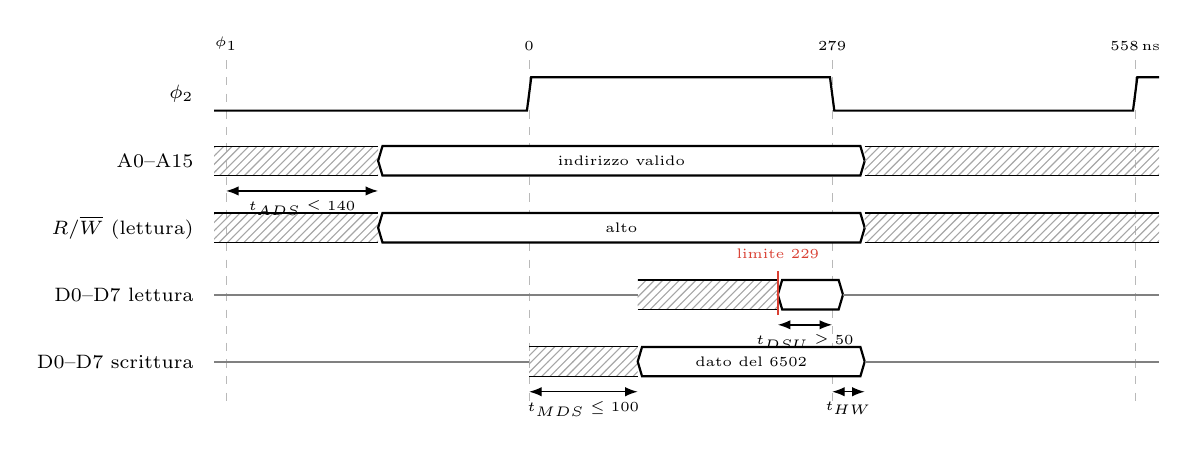
\begin{tikzpicture}[x=0.0138cm, y=0.85cm]
    % griglia
    \foreach \x in {-279,0,279,558} \draw[grid] (\x,0.5) -- (\x,-4.6);
    \node[font=\tiny, above] at (-279,0.5) {$\phi_1$};
    \node[font=\tiny, above] at (0,0.5) {$0$};
    \node[font=\tiny, above] at (279,0.5) {$\HnNTSC$};
    \node[font=\tiny, above] at (558,0.5) {$558$\,ns};
    % PHI2
    \node[lbl] at (-300,0) {$\phi_2$};
    \draw[sig] (-290,-0.25) -- (-2,-0.25) -- (2,0.25) -- (277,0.25) -- (281,-0.25) -- (556,-0.25) -- (560,0.25) -- (580,0.25);
    % indirizzo
    \node[lbl] at (-300,-1) {A0--A15};
    \busx{-1}{-290}{-139}
    \busok{-1}{-139}{309}{indirizzo valido}
    \busx{-1}{309}{580}
    \draw[dim] (-279,-1.45) -- node[below, font=\tiny] {$t_{ADS}\le140$} (-139,-1.45);
    % R/W
    \node[lbl] at (-300,-2) {$R/\overline{W}$ (lettura)};
    \busx{-2}{-290}{-139}
    \busok{-2}{-139}{309}{alto}
    \busx{-2}{309}{580}
    % D lettura
    \node[lbl] at (-300,-3) {D0--D7 lettura};
    \busz{-3}{-290}{100}
    \busx{-3}{100}{229}
    \busok{-3}{229}{289}{}
    \busz{-3}{289}{580}
    \draw[dim] (229,-3.45) -- node[below, font=\tiny] {$t_{DSU}\ge50$} (279,-3.45);
    \draw[cBad, line width=0.8pt] (229,-2.65) -- (229,-3.3);
    \node[cBad, font=\tiny, above] at (229,-2.6) {limite \DLtNTSC};
    % D scrittura
    \node[lbl] at (-300,-4) {D0--D7 scrittura};
    \busz{-4}{-290}{0}
    \busx{-4}{0}{100}
    \busok{-4}{100}{309}{dato del 6502}
    \busz{-4}{309}{580}
    \draw[dim] (0,-4.45) -- node[below, font=\tiny] {$t_{MDS}\le100$} (100,-4.45);
    \draw[dim] (279,-4.45) -- node[below, font=\tiny] {$t_{HW}$} (309,-4.45);
  \end{tikzpicture}
  \caption[Ciclo di bus del 6502 a 1,79\,MHz]{Ciclo di bus del 6502 a $1{,}79\MHz$
  (NTSC) in scala, con i parametri della versione a $2\MHz$. Le zone tratteggiate sono
  valori non garantiti; la riga grigia indica il bus in alta impedenza. L'indirizzo è
  valido circa $140\ns$ prima della salita di $\phi_2$; in lettura il dato deve essere
  stabile da $\DLtNTSC\ns$.}
  \label{fig:ciclo6502}
\end{figure}

\section{Il connettore PBI/ECI e la gestione della memoria}

Il connettore PBI degli XL porta il bus indirizzi e dati, $\phi_2$, $R/\overline{W}$,
\sig{IRQ}, \sig{RESET}, \sig{HALT}, \sig{REFRESH} e tre segnali che un dispositivo esterno
usa per sovrapporsi alla memoria interna~\cite[cap.~10]{ahrm}:
\begin{description}
  \item[\sig{EXTSEL}] (attivo basso) disabilita la RAM interna nel ciclo corrente: il
        dispositivo esterno risponde al suo posto;
  \item[\sig{MPD}] (\emph{Math Pack Disable}, attivo basso) disabilita la ROM interna del
        Math Pack a \hex{D800}--\hex{DFFF}: è la finestra in cui un dispositivo PBI
        mappa la propria ROM di gestione;
  \item[\sig{D1XX}] decodifica della pagina \hex{D1xx} riservata ai dispositivi PBI.
\end{description}
La logica di mappatura della memoria (MMU) decide il dispositivo interno da abilitare
solo in base all'indirizzo e allo stato di PORTB~\cite[§3.4]{ahrm}. Un dispositivo
esterno può sovrapporsi alla RAM e, tramite \sig{MPD}, alla sola ROM del Math Pack, ma
non all'I/O né allo spazio della cartuccia.

I dispositivi PBI commerciali (ICD Multi I/O, CSS Black Box, Atari 1090) decodificano
l'indirizzo con logica combinatoria: \sig{EXTSEL} e \sig{MPD} sono quindi validi poche
decine di nanosecondi dopo che l'indirizzo è stabile, cioè ancora durante $\phi_1$. La
documentazione disponibile non fissa un limite temporale esplicito per questi segnali
rispetto alla generazione dei segnali \sig{RAS}/\sig{CAS} della RAM dinamica e alla
selezione delle ROM interne; il punto è discusso nella sezione~\ref{sec:extsel}.

% =============================================================================
\chapter{Architettura hardware del modulo}
\label{cap:hw}
% =============================================================================

\section{Schema a blocchi}

La figura~\ref{fig:blocchi} riassume l'hardware descritto in~\cite{pinmap,hwreq}. Il bus
Atari è a $5\,\mathrm{V}$ TTL, mentre ESP32-S3 e FPGA sono a $3{,}3\,\mathrm{V}$: tutti i
segnali attraversano traslatori di livello 74LVC4245 (otto canali, direzione impostata
da un pin \sig{DIR} e abilitazione \sig{$\overline{\text{OE}}$}).

\begin{figure}[htbp]
  \centering
  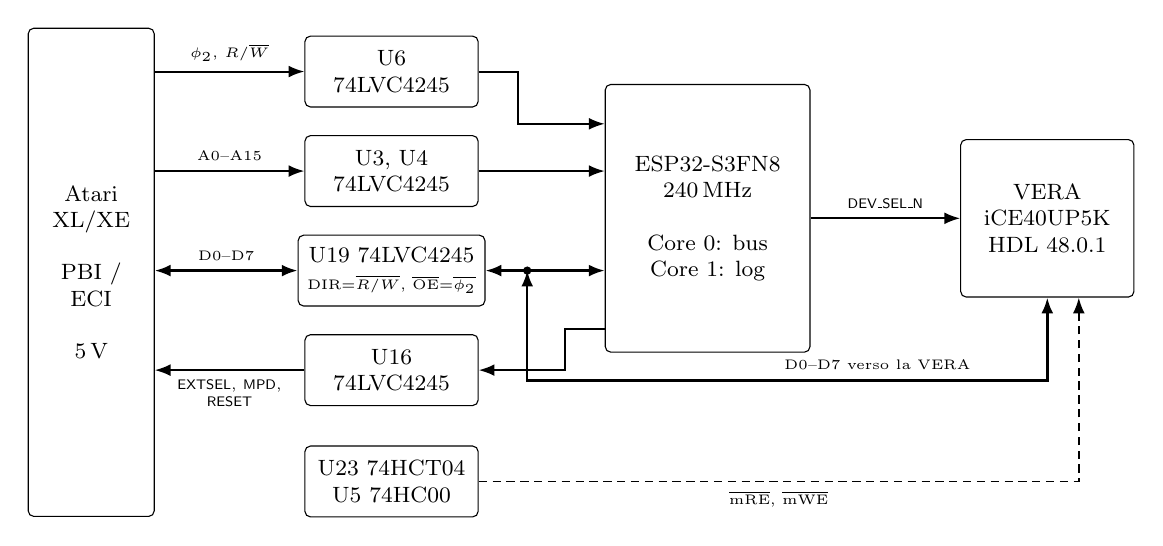
\begin{tikzpicture}[
      blk/.style={draw, rounded corners=2pt, minimum width=2.2cm, minimum height=0.9cm, align=center, font=\footnotesize},
      bus/.style={-{Latex[length=2mm]}, line width=0.7pt},
      bbus/.style={{Latex[length=2mm]}-{Latex[length=2mm]}, line width=0.9pt},
      node distance=0.6cm and 1.0cm]
    \node[blk, minimum height=6.2cm, minimum width=1.6cm] (atari) {Atari\\XL/XE\\ \\ PBI /\\ ECI\\ \\ 5\,V};
    \node[blk, right=1.9cm of atari.north east, anchor=north west, yshift=-0.1cm] (u6) {U6\\ 74LVC4245};
    \node[blk, below=0.35cm of u6] (u34) {U3, U4\\ 74LVC4245};
    \node[blk, below=0.35cm of u34] (u19) {U19 74LVC4245\\ {\tiny DIR=$\overline{R/W}$, $\overline{\text{OE}}$=$\overline{\phi_2}$}};
    \node[blk, below=0.35cm of u19] (u16) {U16\\ 74LVC4245};
    \node[blk, right=1.6cm of u34, minimum height=3.4cm, minimum width=2.6cm, yshift=-0.6cm] (esp) {ESP32-S3FN8\\ 240\,MHz\\ \\ Core 0: bus\\ Core 1: log};
    \node[blk, right=1.9cm of esp, minimum height=2.0cm] (vera) {VERA\\ iCE40UP5K\\ HDL 48.0.1};
    \node[blk, below=0.5cm of u16] (u23) {U23 74HCT04\\ U5 74HC00};
    \draw[bus] (atari.east |- u6) -- node[above, font=\tiny] {$\phi_2$, $R/\overline{W}$} (u6.west);
    \draw[bus] (atari.east |- u34) -- node[above, font=\tiny] {A0--A15} (u34.west);
    \draw[bbus] (atari.east |- u19) -- node[above, font=\tiny] {D0--D7} (u19.west);
    \draw[bus] (u16.west) -- node[below, font=\tiny, align=center] {\sig{EXTSEL}, \sig{MPD},\\ \sig{RESET}} (atari.east |- u16);
    \draw[bus] (u6.east) -- ++(0.5,0) |- ([yshift=1.2cm]esp.west);
    \draw[bus] (u34.east) -- (esp.west |- u34.east);
    \draw[bbus] (u19.east) -- coordinate[pos=0.35] (j) (esp.west |- u19.east);
    \fill (j) circle (1.5pt);
    \draw[bus] ([yshift=-1.4cm]esp.west) -- ++(-0.5,0) |- (u16.east);
    \draw[bus] (esp.east) -- node[above, font=\tiny] {\sig{DEV\_SEL\_N}} (vera.west);
    \draw[bbus] (vera.south) |- node[pos=0.75, above, font=\tiny] {D0--D7 verso la VERA} ($(esp.south)+(0,-0.35)$) -| (j);
    \draw[bus, densely dashed] (u23.east) -| node[pos=0.25, below, font=\tiny] {$\overline{\text{mRE}}$, $\overline{\text{mWE}}$} ([xshift=0.4cm]vera.south);
  \end{tikzpicture}
  \caption[Schema a blocchi del modulo]{Schema a blocchi semplificato del modulo
  Vera-Module-RBL-XE (riferimenti dei componenti dalla netlist del 2026-09-01).}
  \label{fig:blocchi}
\end{figure}

\begin{description}
  \item[U6] traslatore Atari$\to$scheda per $\phi_2$, $R/\overline{W}$, \sig{D1XX},
        \sig{S4}, \sig{S5}, \sig{CCTL}, \sig{REFRESH};
  \item[U3, U4] traslatori del bus indirizzi (A8--A15 e A0--A7);
  \item[U19] traslatore bidirezionale del bus dati. \sig{DIR} è $\overline{R/W}$ e
        $\overline{\text{OE}}$ è $\overline{\phi_2}$, entrambi generati dagli invertitori
        74HCT04 di U23: U19 è abilitato in ogni ciclo, per tutta la fase alta di $\phi_2$;
  \item[U16] traslatore scheda$\to$Atari per \sig{EXTSEL}, \sig{MPD}, \sig{RESET},
        \sig{HALT}, \sig{RD4}, \sig{RD5}, \sig{IRQ};
  \item[U5] porte NAND 74HC00 che generano gli strobe della VERA:
        $\overline{\text{mRE}} = \overline{\phi_2 \cdot R/W}$ e
        $\overline{\text{mWE}} = \overline{\phi_2 \cdot \overline{R/W}}$;
  \item[ESP32-S3FN8] microcontrollore dual core Xtensa LX7 a $240\MHz$ con 8\,MB di flash
        integrata e 512\,KB di SRAM~\cite{esp32s3ds}; il chip select della VERA,
        \sig{DEV\_SEL\_N}, va direttamente alla FPGA a $3{,}3\,\mathrm{V}$;
  \item[VERA] FPGA iCE40UP5K con il firmware VERA 48.0.1; la configurazione è caricata
        da una flash SPI all'uscita dal reset (\sig{CRESET}) e il pin \sig{CDONE} ne
        segnala il completamento.
\end{description}

\section{Assegnazione dei pin dell'ESP32-S3}

L'ESP32-S3FN8 nel package QFN56 offre 45 GPIO, ma sei sono occupati dalla flash interna
e quattro sono pin di strapping letti al reset. Il bus del 6502 richiede 26 segnali di
ingresso (16 indirizzi, 8 dati, $\phi_2$, $R/\overline{W}$) e 3 uscite di controllo: la
tabella~\ref{tab:pin} riporta l'assegnazione~\cite{pinmap}. Restano liberi solo GPIO 47 e
48, troppo pochi per usare i segnali di decodifica hardware presenti sul connettore
(\sig{D1XX}, \sig{S4}, \sig{S5}, \sig{CCTL}): per questo la decodifica dell'indirizzo è
interamente software.

\begin{table}[htbp]
  \centering
  \caption{Assegnazione dei segnali del bus ai GPIO dell'ESP32-S3.}
  \label{tab:pin}
  \small
  \begin{tabular}{llll}
    \toprule
    \textbf{Segnale} & \textbf{GPIO} & \textbf{Registro} & \textbf{Note} \\
    \midrule
    $\phi_2$                & 1          & \code{GPIO.in} bit 1    & e Dedicated GPIO, ingresso 0 \\
    $R/\overline{W}$         & 2          & \code{GPIO.in} bit 2    & \\
    \sig{RAMBO\_EN}         & 3          & \code{GPIO.in} bit 3    & strapping, letto all'avvio \\
    D0--D7                  & 4--11      & \code{GPIO.in} 4--11    & bidirezionale \\
    A0--A7                  & 12--19     & \code{GPIO.in} 12--19   & GPIO 19 = USB D$-$ \\
    A8, A9                  & 20, 21     & \code{GPIO.in} 20--21   & GPIO 20 = USB D$+$ \\
    A12, A13, A10, A11      & 33--36     & \code{GPIO.in1} 1--4    & \\
    A14, A15                & 45, 46     & \code{GPIO.in1} 13--14  & strapping \\
    \sig{ARESET}, \sig{CRESET} & 37, 38  & uscite                 & reset di Atari e VERA \\
    \sig{CDONE}             & 39         & \code{GPIO.in1} bit 7   & configurazione VERA completata \\
    \sig{DEV\_SEL\_N}       & 40         & Dedicated GPIO uscita 0 & chip select VERA \\
    \sig{EXTSEL\_N}         & 41         & Dedicated GPIO uscita 1 & verso il bus via U16 \\
    \sig{MPD}               & 42         & Dedicated GPIO uscita 2 & verso il bus via U16 \\
    UART0 TX, RX            & 43, 44     &                        & log di debug \\
    \bottomrule
  \end{tabular}
\end{table}

Il campionamento dello stato del bus richiede quindi due letture di registri di
periferica: \code{GPIO.in} (GPIO 0--31: $\phi_2$, $R/\overline{W}$, dati, A0--A9) e
\code{GPIO.in1} (GPIO 32--48: A10--A15). I tre segnali di controllo sono invece collegati
al modulo \emph{Dedicated GPIO} dell'ESP32-S3, che la CPU legge e scrive con istruzioni
dedicate (\code{ee.get\_gpio\_in}, \code{ee.wr\_mask\_gpio\_out}) in un ciclo di clock,
senza passare dal bus delle periferiche~\cite{esp32s3trm,idfdedic}.

\section{Logica di traslazione e ritardi}

La tabella~\ref{tab:glue} riporta i ritardi usati nel modello. I valori minimo e massimo
vengono dai datasheet dei componenti nelle condizioni di alimentazione della scheda; per
il 74HC00 alimentato a $3{,}3\,\mathrm{V}$ il datasheet fornisce solo i valori a $2$ e
$4{,}5\,\mathrm{V}$ e quelli in tabella sono interpolati. Il valore per la FPGA è una
stima del percorso pad--logica--pad dell'iCE40UP5K per un'uscita combinatoria.

\begin{table}[htbp]
  \centering
  \caption{Ritardi della logica di interfaccia usati nel modello.}
  \label{tab:glue}
  \begin{tabular}{llccc}
    \toprule
    \textbf{Componente} & \textbf{Percorso} & \textbf{min} & \textbf{tip} & \textbf{max} \\
    \midrule
    74LVC4245A~\cite{lvc4245} & propagazione $5\leftrightarrow3{,}3\,\mathrm{V}$ & 1{,}0 & 4{,}0 & 6{,}5 \\
    74LVC4245A               & disabilitazione uscita                          & 1{,}0 & 4{,}0 & 8{,}0 \\
    74HCT04~\cite{hct04}     & propagazione a $5\,\mathrm{V}$                  & 4     & 10    & 24 \\
    74HC00~\cite{hc00}       & propagazione a $3{,}3\,\mathrm{V}$ (interp.)    & 5     & 12    & 30 \\
    iCE40UP5K~\cite{ice40}   & pad $\to$ logica $\to$ pad (stima)              & 6     & 10    & 15 \\
    ESP32-S3                 & sincronizzatore di ingresso GPIO                & 0     & 12{,}5 & 25 \\
    ESP32-S3                 & uscita GPIO verso il pad                        & 2     & 4     & 6 \\
    \bottomrule
  \end{tabular}\\[2pt]
  {\footnotesize Valori in nanosecondi.}
\end{table}

% =============================================================================
\chapter{Protocollo PBI ed espansione RAMbo 320K}
\label{cap:pbi}
% =============================================================================

\section{Il dispositivo PBI}

\subsection{Selezione tramite \hex{D1FF}}

Più dispositivi PBI possono essere collegati in catena. Il registro \hex{D1FF} (PDVS in
scrittura) seleziona il dispositivo attivo: ogni dispositivo è associato a un bit e
scrivere un valore con il proprio bit a 1 lo seleziona, scrivere \hex{00} deseleziona
tutti~\cite[§10.2]{ahrm}. Il registro non esiste nel computer: ogni dispositivo lo
implementa catturando le scritture all'indirizzo. Il modulo usa il bit 7
(\code{PBI\_DEV\_ID = 0x80}) e, come richiede la regola PBI, considera solo il proprio
bit: \code{selected = (data \& 0x80) != 0}.

Quando un dispositivo è selezionato:
\begin{itemize}
  \item la sua ROM appare a \hex{D800}--\hex{DFFF} al posto del Math Pack (\sig{MPD});
  \item la pagina \hex{D1xx} e l'area \hex{D600}--\hex{D7FF} appartengono a lui
        (\sig{EXTSEL});
\end{itemize}
quando non è selezionato non deve rispondere a nessuno di questi indirizzi, così da
poter convivere con altri dispositivi PBI. Nel modulo i registri della VERA occupano
\hex{D100}--\hex{D11F} e sono quindi accessibili solo con la scheda selezionata
(tabella~\ref{tab:mappa}).

\subsection{La ROM di gestione}

All'avvio il sistema operativo XL/XE seleziona a turno ogni bit di \hex{D1FF}, verifica
l'intestazione della ROM e, se valida, chiama la routine di inizializzazione del
dispositivo. La ROM del modulo (\code{vera\_pbi\_handler.s}, 2\,KB assemblati con
\code{ca65} all'indirizzo \hex{D800}) espone l'intestazione richiesta: \hex{D803} =
\hex{80} (il bit del dispositivo), \hex{D80B} = \hex{91} (firma), \hex{D80C} = \code{'V'},
e i vettori \hex{D805} (SIO, che restituisce \enquote{non gestito}) e \hex{D808} (IRQ).
Ogni lettura di questi byte è un ciclo di lettura servito dall'ESP32: la correttezza
temporale di questi cicli (sezione~\ref{sec:lettura-esp}) è quindi la condizione perché
la scheda venga riconosciuta.

\subsection{Mappa degli indirizzi}

\begin{table}[htbp]
  \centering
  \caption{Indirizzi gestiti dal firmware in modalità PBI.}
  \label{tab:mappa}
  \begin{tabular}{llll}
    \toprule
    \textbf{Intervallo} & \textbf{Condizione} & \textbf{Segnali} & \textbf{Dato} \\
    \midrule
    \hex{D100}--\hex{D11F} & scheda selezionata & \sig{EXTSEL}, \sig{DEV\_SEL\_N} & VERA \\
    \hex{D120}--\hex{D1FE} & scheda selezionata & \sig{EXTSEL}             & non pilotato \\
    \hex{D1FF}             & scrittura          & ---                      & latch di selezione \\
    \hex{D301}, \hex{D303} & scrittura          & ---                      & osservazione PIA \\
    \hex{D600}--\hex{D7FF} & scheda selezionata & \sig{EXTSEL}             & ESP32, RAM 512\,B \\
    \hex{D800}--\hex{DFFF} & scheda selezionata & \sig{MPD}                & ESP32, ROM 2\,KB \\
    \hex{4000}--\hex{7FFF} & RAMbo attiva       & \sig{EXTSEL}             & ESP32, banco 16\,KB \\
    \bottomrule
  \end{tabular}
\end{table}

In modalità CCTL (cartuccia, \code{VERA\_BOARD\_IS\_PBI = 0}) il latch è a \hex{D5FF} e i
registri della VERA occupano \hex{D500}--\hex{D5FE}; non ci sono ROM e RAM PBI.

\section{L'espansione RAMbo 320K}

\subsection{Bank switching tramite PORTB}

Negli XL/XE la porta B della PIA 6520 (\hex{D301}, PORTB) non serve più ai joystick ma
controlla la mappa della memoria: il bit 0 abilita la ROM del sistema operativo, il bit 1
il BASIC, il bit 7 la ROM di autotest a \hex{5000}--\hex{57FF}~\cite[§3.4]{ahrm}. Il
130XE usa i bit 2--5 per un'espansione da 64\,KB vista attraverso la finestra
\hex{4000}--\hex{7FFF}.

L'espansione \enquote{320K Rambo} usa i bit 2, 3, 5 e 6 di PORTB per selezionare uno
di 16 banchi da 16\,KB e il bit 4 per abilitare la finestra: $64 + 16 \times 16 =
320$\,KB~\cite[§3.5]{ahrm}. Poiché il bit 5 serve per il numero di banco, CPU e ANTIC
vedono sempre lo stesso banco: non esiste l'accesso separato di ANTIC del 130XE. Il
firmware calcola il banco come
\begin{equation}
  \text{banco} = \big((\text{PORTB} \gg 2) \;\&\; 3\big) \;|\; \big((\text{PORTB} \gg 3) \;\&\; \text{0x0C}\big)
\end{equation}
che corrisponde alla configurazione \enquote{320K Rambo} documentata per Altirra
(\enquote{PORTB bits 2, 3, 5, and 6 control bank; bit 4 controls CPU+ANTIC
access}~\cite[§11]{ahrm}). Poiché l'ESP32 non distingue i cicli della CPU da quelli di
DMA di ANTIC (non osserva \sig{HALT}), risponde a entrambi con lo stesso banco: è
esattamente il comportamento della RAMbo 320K.

\begin{table}[htbp]
  \centering
  \caption{Valori di PORTB per i 16 banchi (bit 0, 1 e 7 a 1, bit 4 a 0).}
  \label{tab:banchi}
  \small
  \begin{tabular}{cc@{\hspace{1.5em}}cc@{\hspace{1.5em}}cc@{\hspace{1.5em}}cc}
    \toprule
    \textbf{Banco} & \textbf{PORTB} & \textbf{Banco} & \textbf{PORTB} & \textbf{Banco} & \textbf{PORTB} & \textbf{Banco} & \textbf{PORTB} \\
    \midrule
    0 & \hex{83} & 4 & \hex{A3} & 8  & \hex{C3} & 12 & \hex{E3} \\
    1 & \hex{87} & 5 & \hex{A7} & 9  & \hex{C7} & 13 & \hex{E7} \\
    2 & \hex{8B} & 6 & \hex{AB} & 10 & \hex{CB} & 14 & \hex{EB} \\
    3 & \hex{8F} & 7 & \hex{AF} & 11 & \hex{CF} & 15 & \hex{EF} \\
    \bottomrule
  \end{tabular}
\end{table}

\subsection{Osservazione passiva della PIA}

La PIA fisica resta sulla scheda madre e risponde normalmente a \hex{D301} e
\hex{D303}: l'ESP32 non la emula ma ne \emph{osserva} le scritture. A \hex{D301} la PIA
espone due registri diversi, il registro di uscita e il registro di direzione (DDR),
selezionati dal bit 2 del registro di controllo PBCTL (\hex{D303}). Sul bus le due
scritture sono indistinguibili; il firmware tiene quindi una copia di PBCTL e aggiorna
la propria copia di PORTB solo quando il bit 2 di PBCTL è a 1. La tabella~\ref{tab:osinit}
mostra la sequenza tipica del sistema operativo.

\begin{table}[htbp]
  \centering
  \caption{Inizializzazione della PIA da parte del sistema operativo e reazione del firmware.}
  \label{tab:osinit}
  \begin{tabular}{clll}
    \toprule
    \textbf{Passo} & \textbf{Scrittura} & \textbf{PIA} & \textbf{Firmware} \\
    \midrule
    1 & \hex{00} $\to$ \hex{D303} & DDR selezionato a \hex{D301} & \code{pbctl = 0x00} \\
    2 & \hex{FF} $\to$ \hex{D301} & tutti i pin in uscita           & ignorata \\
    3 & \hex{34} $\to$ \hex{D303} & registro di uscita a \hex{D301} & \code{pbctl = 0x34} \\
    4 & \hex{NN} $\to$ \hex{D301} & nuova mappa di memoria          & \code{portb = 0xNN}, tabella aggiornata \\
    \bottomrule
  \end{tabular}
\end{table}

% =============================================================================
\chapter{Architettura del firmware}
\label{cap:fw}
% =============================================================================

\section{Divisione del lavoro fra i due core}

Il firmware è un'applicazione Arduino su ESP-IDF e FreeRTOS. Il core 0 esegue solo il
task \code{MonitorTask}, con la priorità massima, che non cede mai la CPU; il core 1
esegue \code{setup()} e \code{loop()}, quest'ultimo dedicato a stampare sulla seriale gli
eventi prodotti dal core 0. Gli eventi passano attraverso un buffer circolare senza lock
(un produttore, un consumatore): l'inserimento costa poche istruzioni, mentre
\code{xQueueSend()} richiedeva circa $1\us$ e faceva perdere i cicli di bus successivi.

\section{Sequenza di avvio}

\begin{enumerate}
  \item \code{setup()} porta subito a livello basso \sig{ARESET} e \sig{CRESET}: Atari e
        VERA restano in reset per tutta l'inizializzazione;
  \item legge \sig{RAMBO\_EN} (GPIO 3) per sapere se l'emulazione RAMbo è abilitata e
        costruisce le tabelle di decodifica;
  \item \code{MonitorTask} rilascia \sig{CRESET}, attende \sig{CDONE} (timeout $5\,\mathrm{s}$),
        attende ancora $1\,\mathrm{ms}$ per il reset interno della VERA e rilascia
        \sig{ARESET}: da questo momento il bus è attivo e il ciclo principale deve
        rispondere a ogni ciclo di $\phi_2$.
\end{enumerate}

\section{Decodifica a tabelle}

Confrontare l'indirizzo con gli intervalli della tabella~\ref{tab:mappa} a ogni ciclo
costava circa 95 istruzioni. La versione attuale precalcola tutto ciò che dipende dalla
pagina (A8--A15) e dallo stato della scheda (selezionata o no, RAMbo attiva o no) in
quattro tabelle da 256 voci (\code{bus\_decode.h}). L'indice di pagina si ottiene dai due
campioni dei registri GPIO senza riordinare i bit:
\begin{lstlisting}[language=C, caption={Indice di pagina dai registri GPIO (\code{bus\_decode.h}).}]
static inline uint32_t bus_page_idx(uint32_t lo, uint32_t hi)
{
    return ((lo >> 20) & 0x03u) | ((hi << 1) & 0x3Cu) | ((hi >> 7) & 0xC0u);
}
\end{lstlisting}
Ogni voce contiene nei bit 0--2 i livelli di \sig{DEV\_SEL\_N}, \sig{EXTSEL\_N} e
\sig{MPD}, pronti per \code{ee.wr\_mask\_gpio\_out}, e nei bit 3--7 le azioni:
\code{CT\_SLOW} (la decisione dipende anche da A0--A7, solo per \hex{D1xx}/\hex{D5xx}),
\code{CT\_DRIVE} (pilotare il bus in lettura), \code{CT\_RAMBO} (aggiungere l'offset del
banco), \code{CT\_WR\_MEM} (memorizzare il dato in scrittura), \code{CT\_WR\_REG}
(latch o osservazione della PIA). Il passaggio fra gli stati cambia solo il puntatore
alla tabella corrente. La logica non dipende da ESP-IDF ed è verificata sul PC contro la
versione a confronti di intervalli per tutti i 65\,536 indirizzi e i quattro stati.

\section{Il ciclo principale}
\label{sec:loop}

La figura~\ref{fig:flusso} mostra il flusso di un ciclo di bus e il
listato~\ref{lst:loop} il codice sorgente.

\begin{figure}[htbp]
  \centering
  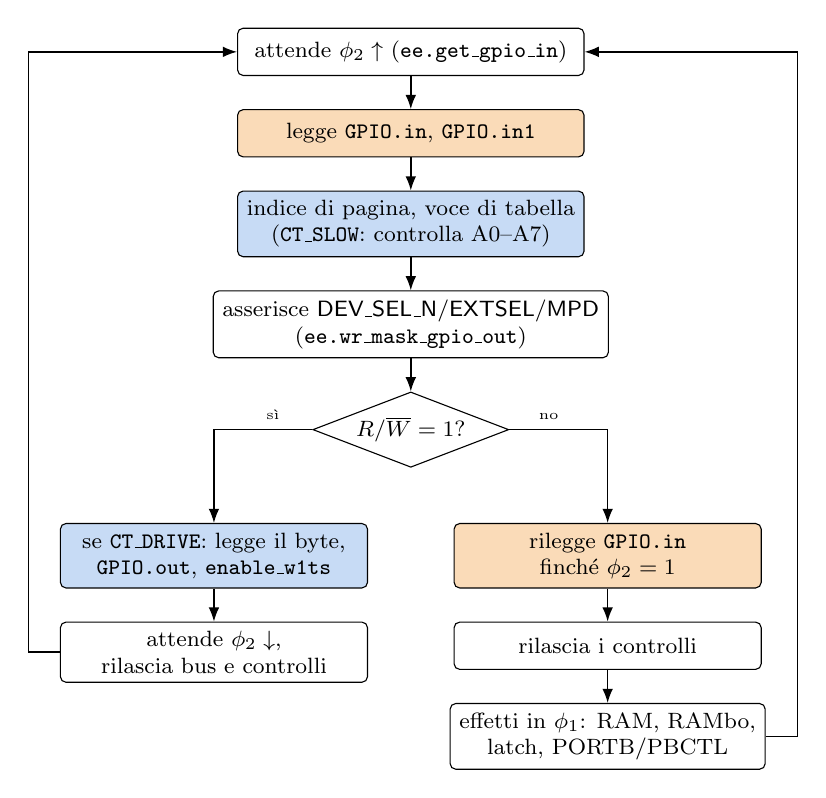
\begin{tikzpicture}[
      node distance=0.42cm,
      box/.style={draw, rounded corners=2pt, align=center, font=\footnotesize, minimum width=4.4cm, minimum height=0.6cm},
      dec/.style={draw, diamond, aspect=2.6, align=center, font=\footnotesize, inner sep=1pt},
      arr/.style={-{Latex[length=1.8mm]}, line width=0.5pt}]
    \node[box] (w) {attende $\phi_2\uparrow$ (\code{ee.get\_gpio\_in})};
    \node[box, below=of w, fill=cApb!40] (r) {legge \code{GPIO.in}, \code{GPIO.in1}};
    \node[box, below=of r, fill=cAlu!40] (d) {indice di pagina, voce di tabella\\ (\code{CT\_SLOW}: controlla A0--A7)};
    \node[box, below=of d] (c) {asserisce \sig{DEV\_SEL\_N}/\sig{EXTSEL}/\sig{MPD}\\ (\code{ee.wr\_mask\_gpio\_out})};
    \node[dec, below=of c] (rw) {$R/\overline{W}=1$?};
    \node[box, below=0.7cm of rw, xshift=-2.5cm, minimum width=3.9cm, fill=cAlu!40] (dr) {se \code{CT\_DRIVE}: legge il byte,\\ \code{GPIO.out}, \code{enable\_w1ts}};
    \node[box, below=of dr, minimum width=3.9cm] (wf) {attende $\phi_2\downarrow$,\\ rilascia bus e controlli};
    \node[box, below=0.7cm of rw, xshift=2.5cm, minimum width=3.9cm, fill=cApb!40] (sm) {rilegge \code{GPIO.in}\\ finché $\phi_2=1$};
    \node[box, below=of sm, minimum width=3.9cm] (rel) {rilascia i controlli};
    \node[box, below=of rel, minimum width=3.9cm] (fx) {effetti in $\phi_1$: RAM, RAMbo,\\ latch, PORTB/PBCTL};
    \draw[arr] (w) -- (r); \draw[arr] (r) -- (d); \draw[arr] (d) -- (c); \draw[arr] (c) -- (rw);
    \draw[arr] (rw.west) -| node[above, font=\tiny, pos=0.2] {sì} (dr.north);
    \draw[arr] (rw.east) -| node[above, font=\tiny, pos=0.2] {no} (sm.north);
    \draw[arr] (dr) -- (wf); \draw[arr] (sm) -- (rel); \draw[arr] (rel) -- (fx);
    \draw[arr] (wf.west) -- ++(-0.4,0) |- (w.west);
    \draw[arr] (fx.east) -- ++(0.4,0) |- (w.east);
  \end{tikzpicture}
  \caption{Flusso del ciclo principale di \code{MonitorTask} per un ciclo di bus.}
  \label{fig:flusso}
\end{figure}

\begin{lstlisting}[language=C++, caption={Ciclo principale di \code{MonitorTask} (estratto di \code{main.cpp}).}, label={lst:loop}]
for (;;)
{
    while (!(cpu_ll_read_dedic_gpio_in() & DEDIC_IN_PHI2));
    uint32_t g_lo = GPIO.in;
    uint32_t g_hi = GPIO.in1.val;

    uint32_t idx  = bus_page_idx(g_lo, g_hi);
    uint32_t c    = ctrl_cur[idx];
    uint32_t off8 = (g_lo >> 12) & 0xFFu;
    if (c & CT_SLOW)
        c = bus_slow_ctrl(c, off8, selected, is_pbi);

    cpu_ll_write_dedic_gpio_mask(DEDIC_OUT_CTRL_MASK, c);

    if (g_lo & (1UL << PIN_RW))
    {
        if (c & CT_DRIVE)
        {
            const uint8_t *p = bus_rd_base[idx];
            if (c & CT_RAMBO)
                p += rambo_off;
            bus_drive(p[off8]);          /* GPIO.out + GPIO.enable_w1ts */
        }
        while (cpu_ll_read_dedic_gpio_in() & DEDIC_IN_PHI2);
        if (c & CT_DRIVE)
            bus_release();
        cpu_ll_write_dedic_gpio_mask(DEDIC_OUT_CTRL_MASK, DEDIC_OUT_CTRL_IDLE);
        continue;
    }

    uint32_t last = g_lo, now;
    while ((now = GPIO.in) & (1UL << PIN_PHI2))
        last = now;
    cpu_ll_write_dedic_gpio_mask(DEDIC_OUT_CTRL_MASK, DEDIC_OUT_CTRL_IDLE);
    /* ... effetti della scrittura durante PHI1 ... */
}
\end{lstlisting}

\section{Analisi del codice generato}
\label{sec:disasm}

Il listato~\ref{lst:asm} riporta il codice Xtensa del percorso di lettura di una pagina
servita dall'ESP32 (ROM PBI), estratto dal disassemblato di \code{firmware.elf}. Il
compilatore traduce fedelmente il sorgente: ogni accesso \code{volatile} ai registri
GPIO è preceduto da \code{memw}, che attende il completamento degli accessi precedenti,
per cui le quattro operazioni sulle periferiche (due letture e due scritture) si
susseguono senza sovrapporsi.

\begin{lstlisting}[language=xtensa, caption={Percorso di lettura nel codice generato (indirizzi \code{0x403753a1}--\code{0x40375436}).}, label={lst:asm}]
loop:  ee.get_gpio_in   a2            ; PHI2 nel bit 0
       bbci     a2, 0, loop           ; attesa del fronte di salita
       memw
       l32i.n   a2, a6, 60            ; GPIO.in   (APB)
       memw
       l32i     a8, a6, 64            ; GPIO.in1  (APB)
       ...                            ; 16 istruzioni: indice di pagina,
       l8ui     a8, a8, 0             ;   voce della tabella ctrl_cur[idx]
       ...
       ee.wr_mask_gpio_out a8, a9     ; DEV_SEL_N / EXTSEL / MPD
       bbci     a2, 2, write          ; R/W
       ...                            ; 22 istruzioni: bus_rd_base[idx],
       l8ui     a2, a11, 0            ;   p[off8], lut_drive[byte]
       ...
       memw
       s32i.n   a8, a2, 4             ; GPIO.out        (APB)
       memw
       s32i     a8, a2, 36            ; GPIO.enable_w1ts (APB)
\end{lstlisting}

La tabella~\ref{tab:cicli} riassume il conteggio. Le istruzioni sono contate a un ciclo,
più due cicli di penalità per ogni salto preso e uno per ogni dipendenza di caricamento
non coperta; gli accessi alle periferiche sono indicati separatamente con la latenza
$L_{APB}$, il parametro discusso nella sezione~\ref{sec:lapb}.

\begin{table}[htbp]
  \centering
  \caption{Cicli di CPU lungo i percorsi del ciclo principale (dal disassemblato).}
  \label{tab:cicli}
  \begin{tabular}{lcc}
    \toprule
    \textbf{Tratto} & \textbf{Cicli} & \textbf{Accessi APB} \\
    \midrule
    attesa di $\phi_2$ (\code{ee.get\_gpio\_in} + \code{bbci}) & 3 per iterazione & --- \\
    letture e decodifica fino ai segnali di controllo & \CycDecFast & 2 letture \\
    \quad idem per \hex{D1xx}/\hex{D5xx} (\code{CT\_SLOW}) & \CycDecSlow & 2 letture \\
    lettura del byte e pilotaggio del bus & \CycDrive & 2 scritture \\
    iterazione del campionamento in scrittura & 6 & 1 lettura \\
    \bottomrule
  \end{tabular}
\end{table}

Il conteggio conferma quanto riportato nella documentazione del progetto (16 istruzioni
dopo le letture per arrivare ai segnali di controllo, 26 per \hex{D1xx}) e aggiunge il
dato che mancava: il percorso completo fino al dato sul bus richiede
$\CycDecFast + \CycDrive = 47$ cicli di sola elaborazione, più quattro accessi alle
periferiche, contro i $\CycAvail$ cicli dell'intera fase alta di $\phi_2$.

% =============================================================================
\chapter{Verifica temporale}
\label{cap:timing}
% =============================================================================

\section{Modello}

Tutti i tempi sono misurati dal fronte di $\phi_2$ sul connettore dell'Atari. Un percorso
è la somma di ritardi hardware (tabella~\ref{tab:glue}) e di tempi di esecuzione
(tabella~\ref{tab:cicli}, ciclo di CPU $t_c = 4{,}167\ns$). Per ogni percorso si calcola
il \emph{margine} (\emph{slack}): il limite meno il tempo calcolato. Un margine negativo è
una violazione.

Si considerano due casi:
\begin{description}
  \item[tipico] ritardi tipici, $\phi_2$ simmetrico, attesa del fronte a metà iterazione;
  \item[peggiore] ritardi massimi, sincronizzatore di ingresso a due cicli di APB,
        fronte rilevato all'ultimo ciclo dell'iterazione di attesa, fase alta di $\phi_2$
        ridotta di $10\ns$.
\end{description}

\subsection{La latenza degli accessi alle periferiche}
\label{sec:lapb}

La CPU dell'ESP32-S3 raggiunge i registri GPIO attraverso il bus delle periferiche, che
funziona a $80\MHz$. La latenza di una lettura di \code{GPIO.in} non è specificata nei
documenti di Espressif disponibili: la documentazione del progetto indica circa 6 cicli
di CPU. Nel modello la latenza $L_{APB}$, uguale per letture e scritture, è un parametro
con tre valori di riferimento:
\begin{center}
  \begin{tabular}{lcc}
    \toprule
    \textbf{Scenario} & $L_{APB}$ \textbf{(cicli)} & $L_{APB}$ \textbf{(ns)} \\
    \midrule
    ottimistico (valore del progetto) & \LapbOtt & \LapbNsOtt \\
    nominale                          & \LapbNom & \LapbNsNom \\
    pessimistico                      & \LapbPes & \LapbNsPes \\
    \bottomrule
  \end{tabular}
\end{center}
La sezione~\ref{sec:mis-lapb} descrive come misurarla con un programma di prova sulla
sola scheda ESP32, senza Atari.

\section{Rilevamento del fronte di \texorpdfstring{$\phi_2$}{phi2}}

Il fronte attraversa U6 ($\le6{,}5\ns$) e il sincronizzatore del GPIO ($0$--$25\ns$);
l'iterazione di attesa dura 3 cicli, per cui il fronte è visto con un'incertezza
di $12{,}5\ns$. Il rilevamento richiede quindi $\DetTyp\ns$ nel caso tipico e
$\DetOtt\ns$ nel caso peggiore.

\section{Ciclo di lettura servito dall'ESP32}
\label{sec:lettura-esp}

È il caso delle letture della ROM PBI, della RAM PBI e della finestra RAMbo. Il percorso è
\begin{equation}
  t_{\text{dato}} = t_{\text{ril}} + \big(\CycDecFast + \CycDrive + 4\,L_{APB}\big)\,t_c + t_{\text{pad}} + t_{U19}
\end{equation}
e va confrontato con il limite~\eqref{eq:deadline}. La figura~\ref{fig:lettura-esp}
mostra il ciclo nel caso tipico con la latenza ottimistica, la
tabella~\ref{tab:lettura} tutti gli scenari.

\begin{figure}[htbp]
  \centering
  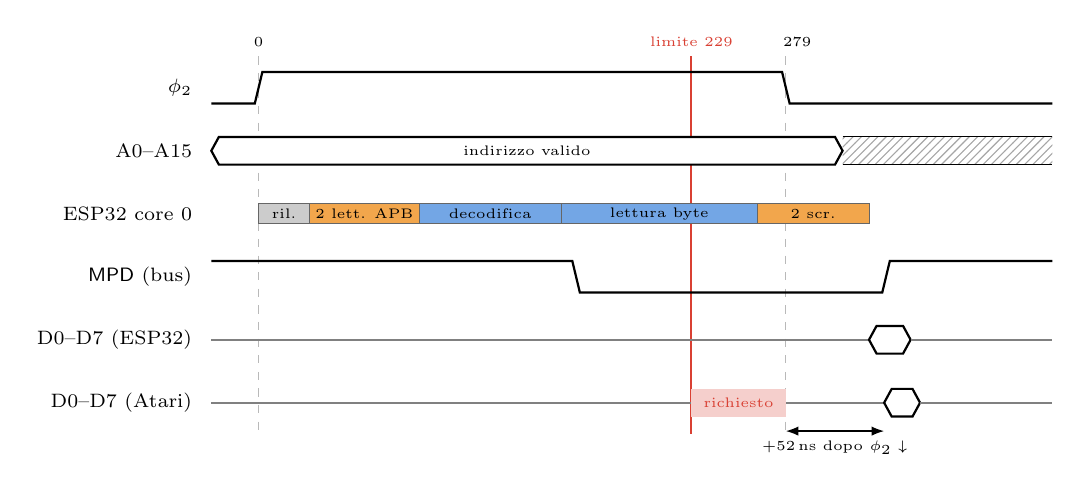
\begin{tikzpicture}[x=0.024cm, y=0.8cm]
    \foreach \x in {0,279} \draw[grid] (\x,0.5) -- (\x,-5.5);
    \draw[cBad, line width=0.7pt] (\DLtNTSC,0.5) -- (\DLtNTSC,-5.5);
    \node[cBad, font=\tiny, above] at (\DLtNTSC,0.5) {limite \DLtNTSC};
    \node[font=\tiny, above] at (0,0.5) {0};
    \node[font=\tiny, above] at (285,0.5) {\HnNTSC};
    % PHI2
    \node[lbl] at (-30,0) {$\phi_2$};
    \draw[sig] (-25,-0.25) -- (-2,-0.25) -- (2,0.25) -- (277,0.25) -- (281,-0.25) -- (420,-0.25);
    % indirizzo
    \node[lbl] at (-30,-1) {A0--A15};
    \busok{-1}{-25}{309}{indirizzo valido}
    \busx{-1}{309}{420}
    % attivita' ESP32
    \node[lbl] at (-30,-2) {ESP32 core 0};
    \act{-2}{0}{\SgDet}{ril.}{cDet}
    \act{-2}{\SgDet}{\SgRd}{2 lett. APB}{cApb}
    \act{-2}{\SgRd}{\SgDec}{decodifica}{cAlu}
    \act{-2}{\SgDec}{\SgLook}{lettura byte}{cAlu}
    \act{-2}{\SgLook}{\SgWr}{2 scr.}{cApb}
    % EXTSEL / MPD
    \node[lbl] at (-30,-3) {\sig{MPD} (bus)};
    \draw[sig] (-25,0.25-3) -- (\SgExt-2,0.25-3) -- (\SgExt+2,-0.25-3) -- (330,-0.25-3) -- (334,0.25-3) -- (420,0.25-3);
    % D sul lato ESP32
    \node[lbl] at (-30,-4) {D0--D7 (ESP32)};
    \busz{-4}{-25}{\SgWr}
    \busok{-4}{\SgWr}{345}{}
    \busz{-4}{345}{420}
    % D lato Atari
    \node[lbl] at (-30,-5) {D0--D7 (Atari)};
    \busz{-5}{-25}{\SgBus}
    \fill[cBad!25] (\DLtNTSC,-5.22) rectangle (279,-4.78);
    \node[font=\tiny, cBad] at (254,-5) {richiesto};
    \busok{-5}{\SgBus}{350}{}
    \busz{-5}{350}{420}
    \draw[dim] (279,-5.45) -- node[below, font=\tiny] {$+\the\numexpr\SgBus-279\relax$\,ns dopo $\phi_2\downarrow$} (\SgBus,-5.45);
  \end{tikzpicture}
  \caption[Lettura servita dall'ESP32 (firmware attuale)]{Lettura della ROM PBI servita
  dall'ESP32, caso tipico con $L_{APB} = \LapbOtt$ cicli. Il dato arriva sul bus
  $\SgBus\ns$ dopo la salita di $\phi_2$, quando il 6502 ha già campionato il bus.}
  \label{fig:lettura-esp}
\end{figure}

\begin{table}[htbp]
  \centering
  \caption{Lettura servita dall'ESP32: istante del dato sul bus e margine.}
  \label{tab:lettura}
  \begin{tabular}{lcccccc}
    \toprule
    & \multicolumn{3}{c}{\textbf{Caso tipico}} & \multicolumn{3}{c}{\textbf{Caso peggiore}} \\
    \cmidrule(lr){2-4}\cmidrule(lr){5-7}
    \textbf{Scenario} & $t_{\text{dato}}$ & \textbf{NTSC} & \textbf{PAL} & $t_{\text{dato}}$ & \textbf{NTSC} & \textbf{PAL} \\
    \midrule
    ottimistico  & \DataEspTOtt & $\SlEspTOttNTSC$ & $\SlEspTOttPAL$ & \DataEspOtt & $\SlEspOttNTSC$ & $\SlEspOttPAL$ \\
    nominale     & \DataEspTNom & $\SlEspTNomNTSC$ & $\SlEspTNomPAL$ & \DataEspNom & $\SlEspNomNTSC$ & $\SlEspNomPAL$ \\
    pessimistico & \DataEspTPes & $\SlEspTPesNTSC$ & $\SlEspTPesPAL$ & \DataEspPes & $\SlEspPesNTSC$ & $\SlEspPesPAL$ \\
    \bottomrule
  \end{tabular}\\[2pt]
  {\footnotesize Tempi e margini in nanosecondi; limite $\DLtNTSC$/$\DLtPAL\ns$ (tipico) e $\DLNTSC$/$\DLPAL\ns$ (peggiore).}
\end{table}

\paragraph{Risultato.} Il percorso viola il setup del 6502 in tutti gli scenari, di
circa $100\ns$ nel più favorevole. Il risultato non dipende dall'incertezza su
$L_{APB}$: anche con accessi alle periferiche istantanei i 47 cicli di elaborazione
($196\ns$) più rilevamento e ritardi di uscita portano il dato a circa $230\ns$, oltre il
limite di $\DLtNTSC\ns$. Le conseguenze sono:
\begin{itemize}
  \item la lettura dell'intestazione della ROM PBI (\hex{D803}, \hex{D80B}) restituisce
        il valore del bus non pilotato (\hex{FF} sugli XL, che hanno resistenze di
        pull-up sul bus dati~\cite[§3.3]{ahrm}): il sistema operativo non riconosce il
        dispositivo;
  \item le letture della finestra RAMbo e della RAM PBI restituiscono dati errati;
  \item il dato pilotato dopo la discesa di $\phi_2$ resta sul bus fino a quando l'ESP32
        rileva il fronte e lo rilascia, cioè fino a circa $60\ns$ nella fase $\phi_1$
        successiva.
\end{itemize}
Il passaggio da NTSC a PAL guadagna soltanto $2{,}6\ns$.

\section{Ciclo di lettura servito dalla VERA}

Per i registri \hex{D100}--\hex{D11F} l'ESP32 deve solo abbassare \sig{DEV\_SEL\_N}: la
VERA ha già il dato pronto (registri e prefetch) e lo porta sul bus attraverso U19. Il
percorso passa per \code{CT\_SLOW} (\CycDecSlow{} cicli e due letture) e prosegue nella FPGA:
\begin{equation}
  t_{\text{VERA}} = t_{\text{ril}} + \big(\CycDecSlow + 2\,L_{APB}\big)\,t_c + t_{\text{pad}} + t_{\text{FPGA}} + t_{U19}.
\end{equation}

\begin{table}[htbp]
  \centering
  \caption{Lettura di un registro VERA: istante del dato sul bus e margine.}
  \label{tab:vera}
  \begin{tabular}{lcccccc}
    \toprule
    & \multicolumn{3}{c}{\textbf{Caso tipico}} & \multicolumn{3}{c}{\textbf{Caso peggiore}} \\
    \cmidrule(lr){2-4}\cmidrule(lr){5-7}
    \textbf{Scenario} & $t_{\text{VERA}}$ & \textbf{NTSC} & \textbf{PAL} & $t_{\text{VERA}}$ & \textbf{NTSC} & \textbf{PAL} \\
    \midrule
    ottimistico  & \DataVeraTOtt & $\SlVeraTOttNTSC$ & $\SlVeraTOttPAL$ & \DataVeraOtt & $\SlVeraOttNTSC$ & $\SlVeraOttPAL$ \\
    nominale     & \DataVeraTNom & $\SlVeraTNomNTSC$ & $\SlVeraTNomPAL$ & \DataVeraNom & $\SlVeraNomNTSC$ & $\SlVeraNomPAL$ \\
    pessimistico & \DataVeraTPes & $\SlVeraTPesNTSC$ & $\SlVeraTPesPAL$ & \DataVeraPes & $\SlVeraPesNTSC$ & $\SlVeraPesPAL$ \\
    \bottomrule
  \end{tabular}\\[2pt]
  {\footnotesize Tempi e margini in nanosecondi.}
\end{table}

\paragraph{Risultato.} La lettura dei registri VERA è al limite: rispetta il setup solo
nel caso tipico con latenza ottimistica, con un margine di $\SlVeraTOttNTSC\ns$ in NTSC.
È il punto in cui la misura di $L_{APB}$ è decisiva.

\section{Cicli di scrittura}

\subsection{Campionamento del dato}

In scrittura il firmware rilegge \code{GPIO.in} finché $\phi_2$ è alto e usa l'ultimo
campione. Il campione contiene nello stesso registro $\phi_2$ e i dati, quindi è
coerente. Il periodo di campionamento è $(L_{APB} + 6)\,t_c$: da $\TsOtt\ns$ a
$\TsPes\ns$. L'ultimo campione con $\phi_2$ alto è preso al più un periodo (più il
sincronizzatore) prima della discesa e deve seguire l'istante in cui il dato del 6502 è
valido ($t_{MDS} + t_{U19}$). Il margine, nel caso peggiore, è di $\SlWrOttNTSC\ns$
(ottimistico), $\SlWrNomNTSC\ns$ (nominale) e $\SlWrPesNTSC\ns$ (pessimistico) in NTSC:
\textbf{il campionamento delle scritture è corretto} in tutti gli scenari.

\subsection{Effetti della scrittura durante \texorpdfstring{$\phi_1$}{phi1}}

Dopo la discesa di $\phi_2$ il firmware applica gli effetti: memorizza il dato nella RAM
PBI o nel banco RAMbo (circa 12 cicli), aggiorna il latch o le copie di PORTB e PBCTL. Il
percorso comune rientra ampiamente nei $279\ns$ di $\phi_1$. Due percorsi meno frequenti
sono più lunghi:
\begin{itemize}
  \item ogni scrittura nelle pagine \hex{D1xx}, \hex{D3xx} e \hex{D5xx}, quindi anche
        \emph{ogni scrittura in un registro della VERA}, chiama \code{bus\_idx\_to\_page()}.
        La funzione è dichiarata \code{static inline} ma il compilatore non l'ha espansa:
        è una chiamata (\code{callx8}) a codice in \emph{flash} (\code{0x42023830}),
        eseguito attraverso la cache delle istruzioni condivisa con il core 1. Un
        \emph{cache miss} costa il caricamento di una linea dalla flash SPI, nell'ordine
        del microsecondo, cioè due o più cicli di bus persi;
  \item il cambio di latch registra un evento (\code{log\_send()} con
        \code{xTaskGetTickCount()}): un centinaio di cicli, che possono far perdere il
        fronte di salita del ciclo seguente.
\end{itemize}
Perdere il fronte non è di per sé un errore: il ciclo seguente viene trattato in
ritardo. È un errore se quel ciclo è una lettura servita dall'ESP32 o una scrittura a un
registro VERA, come avviene nei cicli di scrittura consecutivi su \code{DATA0}.

\subsection{Hold del dato verso la VERA}
\label{sec:hold}

La VERA cattura il dato di scrittura sul fronte di discesa di
\mbox{\texttt{bus\_write = !cs\_n \&\& !wr\_n}}, cioè quando $\overline{\text{mWE}}$ risale dopo la
discesa di $\phi_2$~\cite{hwreq}. Lo stesso fronte di $\phi_2$ disabilita U19 attraverso
U23, e da quel momento il dato al pin della FPGA non è più pilotato. La
figura~\ref{fig:hold} mostra la corsa:
\begin{align}
  t_{\overline{\text{WE}}\uparrow} &= t_{U6} + t_{\text{HC00}}, &
  t_{\text{fine dato}} &= \min\big(t_{HW} + t_{U19},\; t_{\text{HCT04}} + t_{\text{dis},U19}\big).
\end{align}
Il margine di hold è $\HoldTyp\ns$ con i ritardi tipici e $\HoldWorst\ns$ nel caso
peggiore (porte veloci per U23 e U19, lente per U6 e U5): \textbf{la scrittura nei
registri VERA dipende dalla carica residua sulle linee}, non da un margine garantito.
Il problema è indipendente dal firmware ed era già stato segnalato nella documentazione
dell'hardware~\cite[§2.2]{hwreq}.

\begin{figure}[htbp]
  \centering
  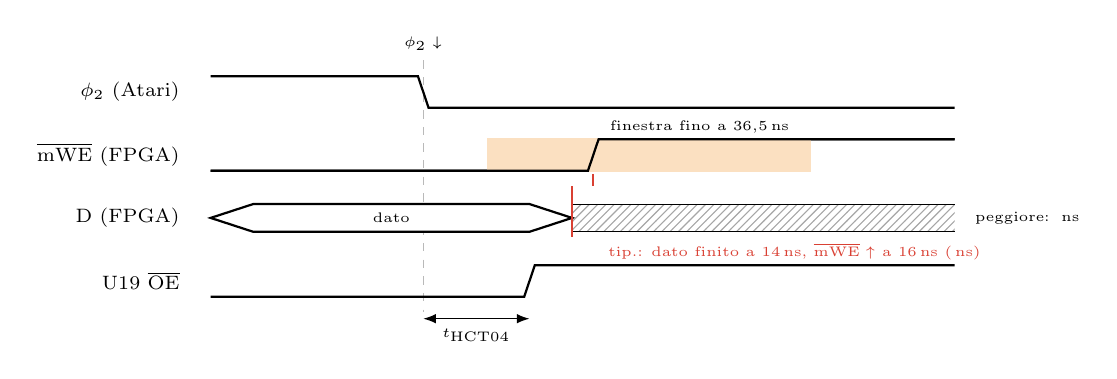
\begin{tikzpicture}[x=0.135cm, y=0.8cm]
    \foreach \x in {0} \draw[grid] (\x,0.5) -- (\x,-3.5);
    \node[font=\tiny, above] at (0,0.5) {$\phi_2\downarrow$};
    \node[lbl] at (-22,0) {$\phi_2$ (Atari)};
    \draw[sig] (-20,0.25) -- (-0.5,0.25) -- (0.5,-0.25) -- (50,-0.25);
    \node[lbl] at (-22,-1) {$\overline{\text{mWE}}$ (FPGA)};
    \draw[sig] (-20,-1.25) -- (16-0.5,-1.25) -- (16+0.5,-0.75) -- (50,-0.75);
    \fill[cApb!35] (6,-1.27) rectangle (36.5,-0.73);
    \draw[sig] (-20,-1.25) -- (16-0.5,-1.25) -- (16+0.5,-0.75) -- (50,-0.75);
    \node[font=\tiny] at (26,-0.55) {finestra fino a $36{,}5\ns$};
    \node[lbl] at (-22,-2) {D (FPGA)};
    \busok{-2}{-20}{14}{dato}
    \busx{-2}{14}{50}
    \node[lbl] at (-22,-3) {U19 $\overline{\text{OE}}$};
    \draw[sig] (-20,-3.25) -- (10-0.5,-3.25) -- (10+0.5,-2.75) -- (50,-2.75);
    \draw[dim] (0,-3.6) -- node[below, font=\tiny] {$t_{\text{HCT04}}$} (10,-3.6);
    \draw[cBad, line width=0.6pt] (14,-1.5) -- (14,-2.3);
    \draw[cBad, line width=0.6pt] (16,-1.3) -- (16,-1.5);
    \node[cBad, font=\tiny, anchor=north west] at (16.5,-2.25) {tip.: dato finito a 14\,ns, $\overline{\text{mWE}}\uparrow$ a 16\,ns ($\HoldTyp$\,ns)};
    \node[font=\tiny, anchor=west] at (51,-2) {peggiore: $\HoldWorst$\,ns};
  \end{tikzpicture}
  \caption[Hold del dato di scrittura verso la VERA]{Hold del dato di scrittura alla
  FPGA (scala: $1\ns = 1{,}6\,\mathrm{mm}$). Il dato smette di essere pilotato quando U19
  si disabilita, mentre la VERA lo cattura alla salita di $\overline{\text{mWE}}$, che può
  arrivare fino a $36{,}5\ns$ dopo la discesa di $\phi_2$.}
  \label{fig:hold}
\end{figure}

\section{Asserzione di \sig{EXTSEL} e \sig{MPD}}
\label{sec:extsel}

Il firmware asserisce \sig{EXTSEL} e \sig{MPD} dopo aver letto l'indirizzo, cioè dopo la
salita di $\phi_2$: al bus arrivano a $\SgExt\ns$ nel caso tipico ottimistico e fino a
$\CtrlPes\ns$ nel caso peggiore pessimistico. Un decodificatore combinatorio li
asserirebbe circa $120\ns$ \emph{prima} della salita di $\phi_2$. Nella fase alta di
$\phi_2$ la logica dell'Atari ha già abilitato la RAM dinamica o la ROM del Math Pack:
\begin{itemize}
  \item in lettura, la RAM o la ROM interna pilota il bus finché \sig{EXTSEL}/\sig{MPD}
        non la disabilita: per alcune decine di nanosecondi due dispositivi pilotano il
        bus dati (contesa);
  \item in scrittura nella finestra RAMbo, se \sig{CAS} della RAM interna è già sceso
        quando arriva \sig{EXTSEL}, la scrittura raggiunge anche la RAM di base a
        \hex{4000}--\hex{7FFF}, che dovrebbe restare nascosta: il contenuto della memoria
        principale viene alterato da scritture destinate ai banchi estesi.
\end{itemize}
L'esatta posizione di \sig{RAS}/\sig{CAS} rispetto a $\phi_2$ dipende dal modello
(800XL con logica discreta, 130XE con FREDDIE) e va misurata. In ogni caso un segnale di
sovrapposizione asserito oltre $150\ns$ dopo la salita di $\phi_2$ è fuori dalla prassi
dei dispositivi PBI esistenti e va considerato non conforme finché la misura non
dimostra il contrario.

\section{Interruzioni sul core 0}
\label{sec:tick}

Il core 0 esegue solo il ciclo principale, ma non ha le interruzioni disabilitate: il
tick di FreeRTOS (\code{CONFIG\_FREERTOS\_HZ = 1000}) interrompe il ciclo una volta al
millisecondo. Ingresso e uscita dall'interruzione (salvataggio della finestra di
registri), gestore del tick ed eventuale riprogrammazione richiedono alcune centinaia di
cicli: con una stima di $1{,}5$--$5\us$ si perdono da 3 a 9 cicli di bus ogni
millisecondo (figura~\ref{fig:tick}).

\begin{figure}[htbp]
  \centering
  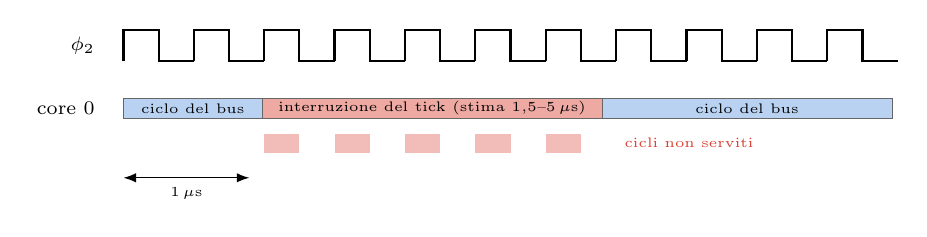
\begin{tikzpicture}[x=1.6cm, y=0.8cm]
    \node[lbl] at (-0.15,0) {$\phi_2$};
    \foreach \i in {0,...,10} {
      \pgfmathsetmacro\a{\i*0.5587}
      \draw[sig] (\a,-0.25) -- ++(0,0.5) -- ++(0.2793,0) -- ++(0,-0.5) -- ++(0.2794,0);
    }
    \node[lbl] at (-0.15,-1) {core 0};
    \act{-1}{0}{1.1}{ciclo del bus}{cAlu!50}
    \act{-1}{1.1}{3.8}{interruzione del tick (stima $1{,}5$--$5\us$)}{cBad!45}
    \act{-1}{3.8}{6.1}{ciclo del bus}{cAlu!50}
    \foreach \i in {2,...,6} {
      \pgfmathsetmacro\a{\i*0.5587}
      \fill[cBad!35] (\a,-1.7) rectangle ++(0.2793,0.3);
    }
    \node[font=\tiny, cBad, anchor=west] at (3.9,-1.55) {cicli non serviti};
    \draw[dim] (0,-2.1) -- node[below, font=\tiny] {$1\us$} (1,-2.1);
  \end{tikzpicture}
  \caption{Effetto dell'interruzione del tick di FreeRTOS sul core 0.}
  \label{fig:tick}
\end{figure}

Sono circa lo $0{,}2$--$0{,}5\,\%$ dei cicli. Per un programma che esegue codice dalla
ROM PBI o dalla finestra RAMbo un ciclo perso è un codice operativo errato, quindi un
blocco entro pochi millisecondi; per un ciclo di scrittura a un registro VERA è una
scrittura persa. Disabilitare le interruzioni sul core 0 non è possibile così com'è:
in ESP-IDF 4.4 il contatore dei tick è aggiornato dal core 0 e il watchdog delle
interruzioni controlla entrambi i core (\code{CONFIG\_ESP\_INT\_WDT\_CHECK\_CPU1 = 1}).
La soluzione è discussa nella sezione~\ref{sec:prop-irq}.

\section{Sintesi grafica}

Le figure~\ref{fig:slack-ntsc} e~\ref{fig:slack-pal} riportano il margine dei percorsi in
funzione di $L_{APB}$: la parte sotto lo zero è la zona di violazione.

\newcommand{\slackplot}[2]{%
  \begin{tikzpicture}
    \begin{axis}[
        width=0.95\textwidth, height=8.2cm,
        xlabel={$L_{APB}$ [cicli di CPU]}, ylabel={margine [ns]},
        xmin=4, xmax=30, ymin=-600, ymax=160,
        grid=both, grid style={gray!20},
        legend columns=2, legend cell align=left,
        legend style={font=\scriptsize, at={(0.5,-0.2)}, anchor=north, draw=gray!50},
        tick label style={font=\scriptsize}, label style={font=\small},
        title={#2}, title style={font=\small}]
      \addplot[draw=none, fill=cBad!8, forget plot] coordinates {(4,-600) (30,-600) (30,0) (4,0)} \closedcycle;
      \addplot[black, line width=0.8pt, forget plot] coordinates {(4,0) (30,0)};
      \addplot[color=cOk!80!black, line width=1.2pt] table[x=lapb, y=wr] {data/slack_#1.dat};
      \addlegendentry{campionamento scrittura (peggiore)}
      \addplot[color=blue!70!black, line width=1.2pt] table[x=lapb, y=prop] {data/slack_#1.dat};
      \addlegendentry{lettura ESP32, ciclo proposto (peggiore)}
      \addplot[color=orange!85!black, line width=1.2pt, dashed] table[x=lapb, y=verat] {data/slack_#1.dat};
      \addlegendentry{lettura VERA (tipico)}
      \addplot[color=orange!85!black, line width=1.2pt] table[x=lapb, y=vera] {data/slack_#1.dat};
      \addlegendentry{lettura VERA (peggiore)}
      \addplot[color=cBad, line width=1.2pt, dashed] table[x=lapb, y=espt] {data/slack_#1.dat};
      \addlegendentry{lettura ESP32, firmware attuale (tipico)}
      \addplot[color=cBad, line width=1.2pt] table[x=lapb, y=esp] {data/slack_#1.dat};
      \addlegendentry{lettura ESP32, firmware attuale (peggiore)}
      \addplot[gray, dashed, forget plot] coordinates {(\LapbOtt,-600) (\LapbOtt,160)};
      \addplot[gray, dashed, forget plot] coordinates {(\LapbNom,-600) (\LapbNom,160)};
      \addplot[gray, dashed, forget plot] coordinates {(\LapbPes,-600) (\LapbPes,160)};
      \node[font=\tiny, gray, anchor=north west, rotate=90] at (axis cs:\LapbOtt,150) {ottimistico};
      \node[font=\tiny, gray, anchor=north west, rotate=90] at (axis cs:\LapbNom,150) {nominale};
      \node[font=\tiny, gray, anchor=north west, rotate=90] at (axis cs:\LapbPes,150) {pessimistico};
    \end{axis}
  \end{tikzpicture}}

\begin{figure}[htbp]
  \centering
  \slackplot{ntsc}{NTSC, $f_{\phi 2} = 1{,}789\,773\MHz$}
  \caption{Margine dei percorsi critici in funzione della latenza APB (NTSC).}
  \label{fig:slack-ntsc}
\end{figure}

\begin{figure}[htbp]
  \centering
  \slackplot{pal}{PAL, $f_{\phi 2} = 1{,}773\,447\MHz$}
  \caption{Margine dei percorsi critici in funzione della latenza APB (PAL).}
  \label{fig:slack-pal}
\end{figure}

\begin{table}[htbp]
  \centering
  \caption{Esito della verifica temporale.}
  \label{tab:esito}
  \begin{tabularx}{\textwidth}{>{\raggedright}p{4.2cm}>{\raggedright}p{2.4cm}X}
    \toprule
    \textbf{Percorso} & \textbf{Esito} & \textbf{Nota} \\
    \midrule
    Lettura ROM/RAM PBI e RAMbo & \textcolor{cBad}{\textbf{non conforme}} & violazione di circa $100$--$370\ns$ in ogni scenario, PAL e NTSC \\
    Lettura registri VERA & \textcolor{orange!80!black}{\textbf{al limite}} & conforme solo con $L_{APB}\approx6$ cicli e ritardi tipici \\
    Campionamento scritture & \textcolor{cOk}{\textbf{conforme}} & margine $\ge\SlWrPesNTSC\ns$ anche nel caso peggiore \\
    Effetti di scrittura in $\phi_1$ & \textcolor{orange!80!black}{\textbf{a rischio}} & chiamata a codice in flash per \hex{D1xx}/\hex{D3xx}/\hex{D5xx} \\
    Hold scrittura VERA & \textcolor{cBad}{\textbf{non conforme}} & $\HoldWorst\ns$ (hardware) \\
    \sig{EXTSEL}/\sig{MPD} & \textcolor{orange!80!black}{\textbf{da misurare}} & asseriti dopo $\phi_2\uparrow$, contesa probabile \\
    Interruzioni sul core 0 & \textcolor{cBad}{\textbf{non conforme}} & 3--9 cicli persi ogni ms \\
    \bottomrule
  \end{tabularx}
\end{table}

% =============================================================================
\chapter{Difetti non temporali}
\label{cap:difetti}
% =============================================================================

L'analisi del codice generato ha messo in luce tre difetti che non dipendono dalle
tempistiche e che impedirebbero il funzionamento anche con un ciclo principale
abbastanza veloce.

\section{Accessi a byte all'area IRAM}
\label{sec:iram-byte}

La ROM PBI (\code{pbi\_driver[]}, dichiarata \code{IRAM\_ATTR}) e l'array della RAMbo
(\code{extended\_rambo\_256k[]}, nella sezione \code{.iram0.bss}) sono collocati agli
indirizzi del bus istruzioni: \code{0x403793b6} e \code{0x40383284}. Il ciclo principale
li legge e li scrive con le istruzioni \code{l8ui} e \code{s8i}. ESP-IDF considera
accessibile a byte solo l'intervallo del bus dati
\code{SOC\_BYTE\_ACCESSIBLE\_LOW}--\code{HIGH} = \code{0x3FC88000}--\code{0x3FD00000}
(\code{soc.h}, funzione \code{esp\_ptr\_byte\_accessible()}): un accesso a 8 bit
all'indirizzo IRAM genera un'eccezione \emph{LoadStoreError} e il riavvio del chip.
Il primo accesso del sistema operativo alla ROM PBI, la lettura di \hex{D803} durante la
scansione dei dispositivi, provocherebbe quindi il blocco del firmware.

\section{Sovrapposizione fra RAMbo e memoria dati}
\label{sec:overlap}

Sull'ESP32-S3 la stessa SRAM è visibile sia dal bus istruzioni
(\code{0x40378000}--\code{0x403DFFFF}) sia dal bus dati
(\code{0x3FC88000}--\code{0x3FCEFFFF}), con uno scostamento costante di \code{0x6F0000}.
Il linker riserva sul bus dati lo spazio occupato dal codice in IRAM con la sezione
\code{.dram0.dummy}, la cui dimensione è calcolata fino al simbolo \code{\_iram\_end}. La
sezione \code{.iram0.bss} creata dall'attributo nel sorgente non è fra quelle previste
dallo script di linker di ESP-IDF: viene collocata dopo \code{\_iram\_end} e non è
contata. Dall'intestazione del file ELF:

\begin{center}
  \small
  \begin{tabular}{lll}
    \toprule
    \textbf{Sezione} & \textbf{Indirizzo} & \textbf{Dimensione} \\
    \midrule
    \code{.dram0.dummy} & \code{0x3FC88000} & \code{0xB284} (fino a \code{\_iram\_end} = \code{0x40383284}) \\
    \code{.dram0.data}  & \code{0x3FC93290} & \code{0x45B8} \\
    \code{.dram0.bss}   & \code{0x3FC97848} & \code{0x14A8} \\
    heap                & da \code{0x3FC98CF0} & \\
    \code{.iram0.bss}   & \code{0x40383284} & \code{0x40000} (alias dati \code{0x3FC93284}--\code{0x3FCD3284}) \\
    \bottomrule
  \end{tabular}
\end{center}

I 256\,KB della RAMbo occupano quindi la stessa memoria fisica di \code{.data},
\code{.bss} e di buona parte dello heap. Con \sig{RAMBO\_EN} alto la chiamata
\code{memset(extended\_rambo\_256k, 0, ...)} in \code{setup()} azzera le variabili
globali, le strutture di FreeRTOS e lo stack del task in esecuzione; anche senza
\code{memset}, ogni scrittura nella finestra RAMbo corromperebbe lo stato del firmware.
Il linker non segnala nulla perché le due viste sono regioni di memoria distinte.

\section{ROM di autotest e finestra RAMbo}
\label{sec:selftest}

Quando il bit 0 di PORTB è a 1 (ROM del sistema abilitata) e il bit 7 è a 0, la ROM di
autotest appare a \hex{5000}--\hex{57FF} con priorità sulla memoria
estesa~\cite[§3.4--3.5]{ahrm}. Le tabelle del firmware considerano solo il bit 4: con
PORTB = \hex{01} (o qualunque valore con bit 0 = 1, bit 4 = 0, bit 7 = 0) l'ESP32
pilota il bus a \hex{5000}--\hex{57FF} insieme alla ROM interna, e \sig{EXTSEL} non può
evitarlo perché disabilita solo la RAM.

\section{Altri punti minori}

\begin{itemize}
  \item La copia di PORTB non tiene conto del DDR: un bit configurato come ingresso
        appare a 1 sui pin della PIA (pull-up), mentre il firmware usa il valore scritto
        nel registro di uscita. Il sistema operativo configura tutti i bit come uscite,
        per cui il caso riguarda solo programmi che modificano il DDR.
  \item Il reset dell'Atari riporta la PIA allo stato iniziale (tutti ingressi, quindi
        PORTB letto come \hex{FF}), ma il firmware conserva l'ultimo valore osservato
        fino alla nuova inizializzazione da parte del sistema operativo.
  \item Il commento all'inizio di \code{main.cpp} descrive ancora i traslatori TXS0108E
        della revisione precedente; la scheda usa 74LVC4245.
\end{itemize}

% =============================================================================
\chapter{Proposte di correzione}
\label{cap:proposte}
% =============================================================================

\section{Correzioni della collocazione in memoria}

Le due correzioni dei difetti delle sezioni~\ref{sec:iram-byte} e~\ref{sec:overlap}
richiedono due righe:

\begin{lstlisting}[language=C++, caption={Collocazione corretta di ROM PBI e RAMbo.}]
/* include/pbi-driver.h */
const uint8_t DRAM_ATTR pbi_driver[] = {            /* era IRAM_ATTR */

/* src/main.cpp: .bss ordinaria nella DRAM, accessibile a byte */
static uint8_t extended_rambo_256k[256 * 1024];     /* senza section(".iram0.bss") */
\end{lstlisting}

La variante è stata compilata: il firmware occupa 289\,376 dei 327\,680 byte della
regione dati (88{,}3\,\%), la RAMbo si trova a \code{0x3FC9784D}, la ROM a
\code{0x3FC94D5C} e lo heap parte da \code{0x3FCD8CF0}. La memoria residua per lo heap è
limitata e va verificata all'avvio (\code{heap\_caps\_get\_free\_size()}).
Nello stesso intervento conviene rendere \code{bus\_idx\_to\_page()}
\code{\_\_attribute\_\_((always\_inline))}, o meglio confrontare direttamente l'indice
di pagina con le costanti precalcolate per \hex{D1}, \hex{D3} e \hex{D5}, eliminando la
chiamata a codice in flash.

\section{Ciclo principale con decodifica durante \texorpdfstring{$\phi_1$}{phi1}}
\label{sec:prop-loop}

Il difetto temporale di fondo è che il firmware inizia a lavorare alla salita di $\phi_2$,
mentre l'indirizzo è stabile da circa $140\ns$. La proposta riorganizza il ciclo in modo
che tutto ciò che dipende dall'indirizzo avvenga in $\phi_1$:
\begin{enumerate}
  \item alla discesa di $\phi_2$ (fine del ciclo precedente) si applicano gli effetti
        della scrittura precedente;
  \item si attende che l'indirizzo sia garantito stabile: $t_{ADS}$ più ritardo di U3/U4
        e sincronizzatore, misurati dal fronte di discesa con il contatore di cicli
        \code{CCOUNT};
  \item si campiona l'indirizzo con \emph{una sola} lettura APB: $\phi_2$,
        $R/\overline{W}$ e A10--A15 passano al modulo Dedicated GPIO, che ha otto canali
        di ingresso e si legge in un ciclo; A0--A9 restano in \code{GPIO.in}. Non serve
        modificare la scheda, perché i canali Dedicated GPIO si collegano a qualunque
        pin attraverso la matrice GPIO;
  \item si decodifica e si asseriscono \sig{EXTSEL}/\sig{MPD}/\sig{DEV\_SEL\_N} prima
        della salita di $\phi_2$, come farebbe un decodificatore combinatorio;
  \item nei cicli di lettura serviti dall'ESP32 si legge il byte da una tabella di
        puntatori per pagina (che include già l'offset del banco RAMbo) e si pilotano i
        pin dati. Il bus Atari resta isolato da U19 fino alla salita di $\phi_2$, per cui
        pilotare i pin in anticipo è sicuro;
  \item alla salita di $\phi_2$ resta solo l'attesa della discesa (lettura) o il
        campionamento del dato (scrittura).
\end{enumerate}

La figura~\ref{fig:proposta} mostra il ciclo risultante nel caso peggiore con latenza
nominale e la tabella~\ref{tab:proposta} i margini.

\begin{figure}[htbp]
  \centering
  \begin{tikzpicture}[x=0.0195cm, y=0.8cm]
    \foreach \x in {-289,0,269} \draw[grid] (\x,0.5) -- (\x,-4.5);
    \draw[cBad, line width=0.7pt] (\DLNTSC,0.5) -- (\DLNTSC,-4.5);
    \node[cBad, font=\tiny, above] at (\DLNTSC,0.5) {limite \DLNTSC};
    \node[font=\tiny, above] at (-289,0.5) {$\phi_2\downarrow$};
    \node[font=\tiny, above] at (0,0.5) {$\phi_2\uparrow$};
    \node[lbl] at (-310,0) {$\phi_2$};
    \draw[sig] (-310,0.25) -- (-291,0.25) -- (-287,-0.25) -- (-2,-0.25) -- (2,0.25) -- (267,0.25) -- (271,-0.25) -- (330,-0.25);
    \node[lbl] at (-310,-1) {A0--A15};
    \busx{-1}{-305}{\PgAddr}
    \busok{-1}{\PgAddr}{299}{indirizzo valido}
    \node[lbl] at (-310,-2) {ESP32 core 0};
    \act{-2}{-280}{-215}{effetti}{cDet}
    \act{-2}{-215}{\PgAddrOk}{attesa $t_{ADS}$}{white}
    \act{-2}{\PgAddrOk}{\PgRd}{1 APB}{cApb}
    \act{-2}{\PgRd}{\PrCtrlNomNTSC}{decodifica}{cAlu}
    \act{-2}{\PrCtrlNomNTSC}{\the\numexpr\PrDataNomNTSC-20\relax}{byte, 2 APB}{cApb}
    \act{-2}{\the\numexpr\PrDataNomNTSC-20\relax}{269}{attesa $\phi_2\downarrow$}{white}
    \node[lbl] at (-310,-3) {\sig{MPD}/\sig{EXTSEL}};
    \draw[sig] (-305,-2.75) -- (\PrCtrlNomNTSC-2,-2.75) -- (\PrCtrlNomNTSC+2,-3.25) -- (300,-3.25) -- (304,-2.75) -- (330,-2.75);
    \node[lbl] at (-310,-4) {D0--D7 (Atari)};
    \busz{-4}{-305}{\PrDataNomNTSC}
    \busok{-4}{\PrDataNomNTSC}{300}{}
    \busz{-4}{300}{330}
    \draw[dim] (\PrDataNomNTSC,-4.45) -- node[below, font=\tiny] {$+\SlPrNomNTSC$\,ns} (\DLNTSC,-4.45);
  \end{tikzpicture}
  \caption[Ciclo principale proposto]{Ciclo di lettura con decodifica durante $\phi_1$,
  caso peggiore in NTSC con $L_{APB} = \LapbNom$ cicli: i segnali di controllo arrivano
  $\PrCtrlNomNTSC\ns$ dopo la salita di $\phi_2$, il dato a $\PrDataNomNTSC\ns$.}
  \label{fig:proposta}
\end{figure}

\begin{table}[htbp]
  \centering
  \caption{Ciclo proposto, caso peggiore: istanti rispetto a $\phi_2\uparrow$ e margine del dato.}
  \label{tab:proposta}
  \begin{tabular}{lcccccc}
    \toprule
    & \multicolumn{3}{c}{\textbf{NTSC}} & \multicolumn{3}{c}{\textbf{PAL}} \\
    \cmidrule(lr){2-4}\cmidrule(lr){5-7}
    \textbf{Scenario} & controlli & dato & margine & controlli & dato & margine \\
    \midrule
    ottimistico  & $\PrCtrlOttNTSC$ & $\PrDataOttNTSC$ & $\SlPrOttNTSC$ & $\PrCtrlOttPAL$ & $\PrDataOttPAL$ & $\SlPrOttPAL$ \\
    nominale     & $\PrCtrlNomNTSC$ & $\PrDataNomNTSC$ & $\SlPrNomNTSC$ & $\PrCtrlNomPAL$ & $\PrDataNomPAL$ & $\SlPrNomPAL$ \\
    pessimistico & $\PrCtrlPesNTSC$ & $\PrDataPesNTSC$ & $\SlPrPesNTSC$ & $\PrCtrlPesPAL$ & $\PrDataPesPAL$ & $\SlPrPesPAL$ \\
    \bottomrule
  \end{tabular}\\[2pt]
  {\footnotesize Valori in nanosecondi.}
\end{table}

Il ciclo proposto rientra nei limiti per latenze fino a circa 15 cicli; nello scenario
pessimistico resta in violazione, perché il campionamento attende il valore massimo di
$t_{ADS}$ e lascia poco più di $100\ns$ prima della salita di $\phi_2$. Anche i segnali
di sovrapposizione arrivano in prossimità della salita di $\phi_2$ e non $120\ns$ prima
come con un decodificatore combinatorio: il miglioramento è grande, ma la conformità
dipende ancora dalla misura di $L_{APB}$ e di $t_{ADS}$ reale.

\section{Isolamento del ciclo principale dalle interruzioni}
\label{sec:prop-irq}

Per eliminare la perdita di cicli della sezione~\ref{sec:tick} il ciclo principale deve
girare a interruzioni disabilitate. In ESP-IDF 4.4 questo richiede:
\begin{itemize}
  \item spostare \code{MonitorTask} sul core 1 e il log sul core 0, che deve continuare
        ad aggiornare il contatore dei tick;
  \item disabilitare nel task le interruzioni fino al livello del watchdog
        (\code{XTOS\_SET\_INTLEVEL}) e alimentare periodicamente il watchdog delle
        interruzioni, oppure compilare il framework con
        \code{CONFIG\_ESP\_INT\_WDT\_CHECK\_CPU1 = n} (Arduino come componente di
        ESP-IDF);
  \item evitare nel ciclo qualunque chiamata a funzioni di FreeRTOS: il timestamp degli
        eventi può essere il registro \code{CCOUNT}.
\end{itemize}

\section{Correzioni minori del firmware}

\begin{itemize}
  \item Aggiungere alle tabelle lo stato \enquote{autotest visibile}
        (\code{(portb \& 0x81) == 0x01}) ed escludere le pagine \hex{50}--\hex{57} dalla
        finestra RAMbo in quello stato (otto tabelle invece di quattro, 2\,KB).
  \item Calcolare il PORTB effettivo come \code{out | \textasciitilde ddr}, osservando
        anche le scritture al DDR.
\end{itemize}

\section{Correzioni hardware}

Restano necessarie le modifiche già individuate nella documentazione della
scheda~\cite{hwreq}, che l'analisi conferma:
\begin{itemize}
  \item abilitare U19 solo nei cicli in cui la scheda risponde o in scrittura, invece che
        in ogni ciclo con $\phi_2$ alto: oggi U19 pilota il bus dati dell'Atari con
        livelli indefiniti in ogni lettura di RAM o ROM interna;
  \item rendere positivo l'hold della scrittura verso la VERA
        (sezione~\ref{sec:hold}), ritardando la disabilitazione di U19 rispetto alla
        salita di $\overline{\text{mWE}}$ e sostituendo il 74HC00 con una porta più
        veloce a $3{,}3\,\mathrm{V}$ (74LVC00);
  \item collegare l'uscita IRQ della VERA, che è push-pull, attraverso uno stadio
        open-drain (74LVC1G07).
\end{itemize}

\section{Alternativa architetturale: ROM, RAM e RAMbo nella FPGA di interfaccia}

Il repository contiene anche un'implementazione dello stesso controllo del bus in VHDL
per una FPGA iCE40UP5K di interfaccia (\code{C6502\_Interface.vhd}), con ROM e RAM PBI
in BRAM e la RAMbo in una SRAM asincrona esterna da $55\ns$. In logica combinatoria la
decodifica segue l'indirizzo di poche decine di nanosecondi, \sig{EXTSEL} e \sig{MPD} sono
validi durante $\phi_1$ e il dato della SRAM arriva sul bus circa $30$--$40\ns$ dopo la
salita di $\phi_2$, con un margine di quasi $200\ns$. Se le misure della
sezione~\ref{sec:mis-lapb} confermassero latenze APB elevate, questa sarebbe la strada
più solida: all'ESP32 resterebbero l'avvio, il reset e la diagnostica.

% =============================================================================
\chapter{Piano di verifica sperimentale}
\label{cap:verifica}
% =============================================================================

\section{Misura della latenza APB}
\label{sec:mis-lapb}

La latenza di \code{GPIO.in} si misura su una scheda ESP32-S3 qualsiasi, senza Atari,
con il contatore di cicli della CPU. Il listato~\ref{lst:bench} esegue 1000 letture e
riporta i cicli medi per lettura; la stessa struttura con \code{GPIO.out} misura le
scritture.

\begin{lstlisting}[language=C++, caption={Misura della latenza di lettura di \code{GPIO.in}.}, label={lst:bench}]
#include <Arduino.h>
#include <soc/gpio_struct.h>
#include <xtensa/hal.h>

static void IRAM_ATTR bench(void)
{
    uint32_t sink = 0;
    portDISABLE_INTERRUPTS();
    uint32_t t0 = xthal_get_ccount();
    for (int i = 0; i < 1000; i++)
        sink += GPIO.in;                /* memw + l32i, come nel firmware */
    uint32_t t1 = xthal_get_ccount();
    portENABLE_INTERRUPTS();
    Serial.printf("GPIO.in: %.2f cicli (sink %u)\n", (t1 - t0) / 1000.0f, sink);
}

void setup() { Serial.begin(115200); delay(500); bench(); }
void loop()  {}
\end{lstlisting}

Il valore misurato, meno i 3--4 cicli di overhead dell'iterazione, sostituisce
\code{SCENARIOS} in \code{timing\_model.py}; ricompilando la tesi si aggiornano tabelle
e grafici. Lo stesso programma, con il core 1 impegnato a stampare sulla seriale, mostra
l'effetto della contesa sul bus delle periferiche.

\section{Misure sul bus con analizzatore logico}

Con l'analizzatore logico (almeno $200\,\mathrm{MS/s}$ per una risoluzione di $5\ns$) e
la scheda collegata all'Atari:
\begin{enumerate}
  \item duty cycle di $\phi_2$ sul connettore, in PAL e NTSC;
  \item $t_{ADS}$ reale: ritardo fra la discesa di $\phi_2$ e la stabilità di A0--A15;
  \item ritardo fra la salita di $\phi_2$ e \sig{DEV\_SEL\_N}, \sig{EXTSEL}, \sig{MPD};
  \item ritardo fra la salita di $\phi_2$ e il dato sul connettore in una lettura di
        \hex{D803}, confrontato con la discesa di $\phi_2$;
  \item posizione di \sig{RAS}/\sig{CAS} della RAM interna rispetto a $\phi_2$ (sonda
        sulla scheda madre) per stabilire il limite reale di \sig{EXTSEL};
  \item hold del dato al pin della FPGA rispetto alla salita di $\overline{\text{mWE}}$;
  \item cicli non serviti: un GPIO libero (47 o 48) commutato a ogni iterazione del
        ciclo principale rende visibili le pause del tick e dei cache miss.
\end{enumerate}

\section{Prove funzionali}

Dopo le misure, i programmi di prova del progetto~\cite{hwreq} verificano il
comportamento complessivo: riconoscimento della ROM PBI all'avvio, rilevamento della
VERA (\code{vera\_detect()}), \code{TESTFX.COM} (atteso 36 PASS), prove della RAMbo con un
programma che scrive e rilegge tutti i 16 banchi controllando che la memoria di base a
\hex{4000}--\hex{7FFF} resti invariata, e \code{TESTIRQ.COM} dopo il montaggio dello
stadio open-drain.

% =============================================================================
\chapter{Conclusioni}
\label{cap:concl}
% =============================================================================

Il modulo Vera-Module-RBL-XE affida a un ESP32-S3 l'intera decodifica del bus di un
Atari XL/XE: registri della VERA, dispositivo PBI ed emulazione della RAMbo 320K. La
logica è corretta: il latch di selezione usa solo il proprio bit come richiede il
protocollo PBI, la scheda non risponde quando non è selezionata, il bank switching segue
la configurazione \enquote{320K Rambo} (bit 2, 3, 5, 6 per il banco, bit 4 per
l'abilitazione di CPU e ANTIC) e l'osservazione di PBCTL distingue correttamente le
scritture al DDR da quelle a PORTB. Anche il campionamento dei cicli di scrittura
rispetta le tempistiche del 6502.

La verifica temporale mostra però che, a $1{,}77$ e a $1{,}79\MHz$, il firmware attuale non
è conforme per i cicli di lettura serviti dall'ESP32: l'elaborazione inizia alla salita
di $\phi_2$ e i 47 cicli di istruzioni più quattro accessi alle periferiche non possono
rientrare nei $279\ns$ della fase alta meno il setup del processore. La differenza fra
PAL e NTSC ($2{,}6\ns$) è irrilevante rispetto al deficit. Le letture dei registri VERA
sono al limite e dipendono dalla latenza APB reale; le interruzioni sul core 0 fanno
perdere alcuni cicli ogni millisecondo. L'analisi del codice generato ha inoltre rivelato
che ROM PBI e RAMbo sono in un'area non accessibile a byte e che la RAMbo si sovrappone
alla memoria dati del firmware: difetti che bloccherebbero la scheda alla prima lettura
della ROM o all'avvio con la RAMbo abilitata.

Le correzioni della collocazione in memoria sono immediate e già verificate in
compilazione. La riorganizzazione del ciclo principale con decodifica durante $\phi_1$,
una sola lettura APB e pilotaggio anticipato del bus porta il margine a circa
$+\SlPrNomNTSC\ns$ con latenza nominale, ma resta dipendente dalle misure. Se le misure
di $L_{APB}$ confermassero valori alti, la soluzione robusta è spostare ROM, RAM e RAMbo
nella FPGA di interfaccia già progettata, lasciando all'ESP32 i compiti non critici.

% =============================================================================
\begin{thebibliography}{99}
% =============================================================================
\bibitem{ahrm} A. Lee, \emph{Altirra Hardware Reference Manual}, versione 07/05/15, 2015.
\bibitem{r6502} Rockwell International, \emph{R6500 Microprocessors (CPU) -- R6502, R6502A},
  data sheet, caratteristiche AC dei cicli di lettura e scrittura.
\bibitem{mos} MOS Technology, \emph{MCS6500 Microcomputer Family Hardware Manual}, 1976.
\bibitem{esp32s3ds} Espressif Systems, \emph{ESP32-S3 Series Datasheet}, v2.2.
\bibitem{esp32s3trm} Espressif Systems, \emph{ESP32-S3 Technical Reference Manual},
  capitoli \enquote{System and Memory}, \enquote{IO MUX and GPIO Matrix} e
  \enquote{Dedicated GPIO}.
\bibitem{idfdedic} Espressif Systems, \emph{ESP-IDF Programming Guide v4.4}:
  \enquote{Dedicated GPIO} e \enquote{Memory Types}; \code{soc/esp32s3/include/soc/soc.h}.
\bibitem{lvc4245} NXP Semiconductors, \emph{74LVC4245A -- Octal dual supply translating
  transceiver; 3-state}, data sheet.
\bibitem{hct04} Texas Instruments, \emph{SN74HCT04 Hex Inverters}, data sheet.
\bibitem{hc00} Texas Instruments, \emph{SN74HC00 Quadruple 2-Input Positive-NAND Gates},
  data sheet.
\bibitem{ice40} Lattice Semiconductor, \emph{iCE40 UltraPlus Family Data Sheet}.
\bibitem{vera} F. van den Hoef, \emph{VERA -- Versatile Embedded Retro Adapter}, HDL
  48.0.1, progetto Commander X16.
\bibitem{rambo} ICD Inc., \emph{RAMBO XL Memory Upgrade -- manuale}.
\bibitem{pinmap} Progetto Vera-Module-RBL-XE, \code{PIN-MAPPING.md} e
  \code{firmware/MCU/README.md}.
\bibitem{hwreq} Progetto Vera-Module-RBL-XE, \code{VERA-ATARI-HW-REQUIREMENTS.md},
  2026-10-06.
\end{thebibliography}

% =============================================================================
\appendix
\chapter{Il modello temporale}
\label{app:modello}
% =============================================================================

Lo script \code{timing\_model.py} contiene tutti i parametri delle
tabelle~\ref{tab:6502}, \ref{tab:glue} e~\ref{tab:cicli} e calcola i percorsi descritti nel
capitolo~\ref{cap:timing}. Produce \code{data/numbers.tex}, con una macro \LaTeX{} per ogni
valore citato nel testo, e i file \code{data/slack\_ntsc.dat} e \code{data/slack\_pal.dat}
per i grafici. Per aggiornare la tesi dopo una misura:
\begin{lstlisting}[language=bash]
python3 timing_model.py      # rigenera data/
latexmk -pdf tesi.tex        # oppure: pdflatex tesi.tex (due volte)
\end{lstlisting}

\end{document}
